%% LyX 2.1.4 created this file.  For more info, see http://www.lyx.org/.
%% Do not edit unless you really know what you are doing.
\documentclass[oneside]{amsart}
\usepackage[latin9]{inputenc}
\setlength{\parskip}{\medskipamount}
\setlength{\parindent}{0pt}
\usepackage{float}
\usepackage{mathtools}
\usepackage{enumitem}
\usepackage{amsbsy}
\usepackage{amstext}
\usepackage{amsthm}
\usepackage{amssymb}
\usepackage{cancel}
\usepackage{graphicx}
\usepackage{esint}

\makeatletter

%%%%%%%%%%%%%%%%%%%%%%%%%%%%%% LyX specific LaTeX commands.
%% Because html converters don't know tabularnewline
\providecommand{\tabularnewline}{\\}

%%%%%%%%%%%%%%%%%%%%%%%%%%%%%% Textclass specific LaTeX commands.
\numberwithin{equation}{section}
\numberwithin{figure}{section}
  \theoremstyle{plain}
  \newtheorem*{cor*}{\protect\corollaryname}
  \theoremstyle{plain}
  \newtheorem*{thm*}{\protect\theoremname}
 \newlist{casenv}{enumerate}{4}
 \setlist[casenv]{leftmargin=*,align=left,widest={iiii}}
 \setlist[casenv,1]{label={{\itshape\ \casename} \arabic*.},ref=\arabic*}
 \setlist[casenv,2]{label={{\itshape\ \casename} \roman*.},ref=\roman*}
 \setlist[casenv,3]{label={{\itshape\ \casename\ \alph*.}},ref=\alph*}
 \setlist[casenv,4]{label={{\itshape\ \casename} \arabic*.},ref=\arabic*}
 \theoremstyle{definition}
 \newtheorem*{defn*}{\protect\definitionname}
  \theoremstyle{plain}
  \newtheorem*{lem*}{\protect\lemmaname}
  \theoremstyle{definition}
  \newtheorem*{example*}{\protect\examplename}

%%%%%%%%%%%%%%%%%%%%%%%%%%%%%% User specified LaTeX commands.

%
\usepackage{amsfonts}
%\usepackage{mathabx}
\usepackage{nopageno}%%%  The following few lines affect the margin sizes. 
\usepackage{bm}
\addtolength{\topmargin}{-.5in}
\setlength{\textwidth}{6in}       
\setlength{\oddsidemargin}{.25in}              
\setlength{\evensidemargin}{.25in}         
  
\setlength{\textheight}{9in}
\renewcommand{\baselinestretch}{1}
\reversemarginpar   
%
%

\makeatother

  \providecommand{\corollaryname}{Corollary}
  \providecommand{\definitionname}{Definition}
  \providecommand{\examplename}{Example}
  \providecommand{\lemmaname}{Lemma}
  \providecommand{\theoremname}{Theorem}
 \providecommand{\casename}{Case}

\begin{document}

\section{Convex Sets}
\begin{enumerate}
\item The set of optima for a min LP is a convex set (just use linearity
of the matrix defining the constraints, i.e. since $Ax\preceq b$
defines the polyhedron).
\item Intersection, Minkowski sum, Minkowski difference, preserve convexity
of sets.
\item Caratheodory's theorem: for a convex set in $\mathbb{R}^{n}$ any
point can be expressed as a convex combination of at most $n+1$ points
(prove using linear independence of differences between points).
\item For $S$ a convex set with non-empty interior, $x_{1}$ in the closure
of $S$ and $x_{2}$ in the interior then the ``weak'' convex combination,
i.e. ($\lambda\in\left(0,1\right)$) is always in the interior.
\item The interior of a convex set is convex and if the interior is non-empty
then so is the closure.
\item For a convex set with non-empty interior $cl\left(int\left(S\right)\right)=cl\left(S\right)$
and $int\left(cl\left(S\right)\right)=int\left(S\right)$.
\end{enumerate}

\section{Hyperplanes}


\subsection{Projection theorem}

Projection theorem: for any closed convex set $S$ and for any point
not in the convex set $y$ there exists a projection $\bar{x}$ of
$y$ onto $S$ and $\bar{x}$ is such that $\left(y-\bar{x}\right)^{\intercal}\left(x-\bar{x}\right)\leq0$
for all $x\in S$, i.e. the plane defined by $\left(y-\bar{x}\right)$
separates $S$ from $y$.
\begin{figure}[H]


\noindent \begin{centering}
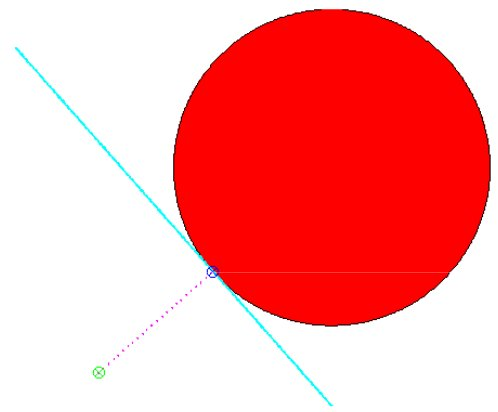
\includegraphics[scale=0.5]{projection_hyperplane}\caption{Projection theorem}

\par\end{centering}

\end{figure}

\begin{proof}
We seek to minimize $\left\Vert x-y\right\Vert $ over $x\in S$.
This is equivalent to minimizing over the set
\[
\left\{ x\big|\left\Vert x-y\right\Vert \leq\left\Vert x-w\right\Vert \right\} 
\]
for some $w\in S$. Why? Because $\left\{ x\big|\left\Vert x-y\right\Vert \leq\left\Vert x-w\right\Vert \right\} \subset S$
and the $\bar{x}$ that minimizes $\left\Vert x-y\right\Vert $ is
definitely in it (since it's smaller than all $\left\Vert x-y\right\Vert $).
This is a bounded closed set (since $S$ is closed) and norms are
continuous and so by extreme value theorem there exists a minimum.
$\bar{x}$ is unique: suppose there exist two such points $\bar{x}_{1},\bar{x}_{2}$.
Then
\begin{align*}
0 & <\left\Vert \left(\bar{x}_{1}-y\right)-\left(\bar{x}_{2}-y\right)\right\Vert ^{2}\\
 & =2\left\Vert \bar{x}_{1}-y\right\Vert ^{2}+2\left\Vert \bar{x}_{2}-y\right\Vert ^{2}-4\left\Vert \frac{1}{2}\left[\left(\bar{x}_{1}-y\right)-\left(\bar{x}_{2}-y\right)\right]\right\Vert ^{2}\\
 & =2\left\Vert \bar{x}_{1}-y\right\Vert ^{2}+2\left\Vert \bar{x}_{2}-y\right\Vert ^{2}-4\left\Vert \frac{\left(\bar{x}_{1}+\bar{x}_{2}\right)}{2}-y\right\Vert ^{2}\\
 & =2\left\Vert \bar{x}_{1}-y\right\Vert ^{2}+2\left\Vert \bar{x}_{2}-y\right\Vert ^{2}-4\left\Vert \hat{x}-y\right\Vert ^{2}
\end{align*}
Since $\left\Vert \bar{x}_{1}-y\right\Vert =\left\Vert \bar{x}_{2}-y\right\Vert =s$
rearranging we have $\left\Vert \hat{x}-y\right\Vert <s$ contradicting
that $x_{1},x_{2}$ are minimal projections. 
\begin{cor*}
Let $S$ be the column space of some matrix $A$ and $y\notin S$.
Then for the projection $\bar{z}$ it's the case that $\left(y-\bar{z}\right)\perp z$
for all $z\in col\left(A\right)$ and $A^{\intercal}\bar{z}=A^{\intercal}y$
(i.e. the projection is the perpendicular projector).
\end{cor*}


\begin{cor*}
Least squares.
\end{cor*}
\end{proof}
\textbf{Improper separation} is when possibly both sets are in the
the separating hyperplane. \textbf{Proper separation} is when the
union of the two sets isn't contained in the separating hyperplane.
\textbf{Strict separation }is when the convex sets don't intersect
the separating hyperplane (but their closures might). \textbf{Strong
separation} is when there's ``fat'' in between the sets and the
hyperplane.

Point-to-set separation: for any non-empty closed convex set $S$
and $y\notin S$ there's a separating hyperplane. Proof: use the projection
theorem to find the projection. Keep in mind the obtuseness ($\left(y-\bar{x}\right)^{\intercal}\left(x-\bar{x}\right)\leq0$
says that every vector from $x\in S$ to $\bar{x}$ is obtuse to the
normal vector to the separating hyperplane $p=y-\bar{x}$).
\begin{cor*}
Every closed convex set is the intersection of halfspaces (take all
the separation hyperplanes and intersection the half spaces that the
set is in).
\end{cor*}

\begin{cor*}
Let $S$ be nonempty and $y$ not in the closure of the convex hull
of $S$. Then you can stronly separate.
\end{cor*}

\subsection{LP Duality}
\begin{thm*}
Farkas' lemma: exactly one of the two following systems has a solution
\begin{align*}
x\text{ s.t. } & Ax\preceq0\text{ and }c^{\intercal}x>0\\
y\text{ s.t. } & A^{\intercal}y=c\text{ and }y\succeq0
\end{align*}
The intuition here is if the columns of $A^{\intercal}$ by $a_{1},\dots,a_{m}$
the second system has a solution iff $c$ lies in the conic cone???
of $a_{1},\dots,a_{m}$. Apparently a convex cone is a cone closed
under conic combinations and a cone is any set closed under positive
scalings. If $c$ doesn't lie in the cone then the polyhedral convex
cone\footnote{Why is this a polyhedral cone? Well $x$ that satisfies $Ax\preceq b$
is the intersection of half-spaces (think hyperplanes defined by the
rows of $A$). If $b=0$ then all of those halfspaces go through the
origin.}$Ax\preceq0$ and the halfspace $c^{\intercal}x>0$ have a nonempty
intersection. Note that cone defined by this system is actually the
polar of the vectors themselves (since these vectors actually define
the \textbf{normals} to the plane). This is basically all about polar
cones. Either a vector is in the convex cone or there exists a vector
in the polar cone that makes an accute angle with it (though not necessarily
in the polar cone). 
\begin{figure}[H]


\noindent \begin{centering}
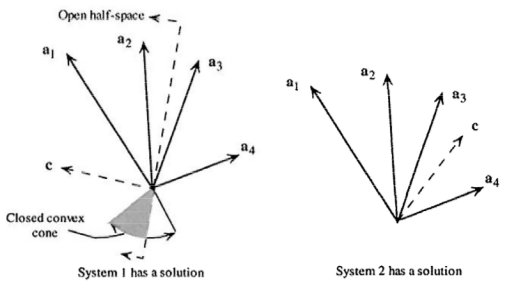
\includegraphics[scale=0.7]{farkas}\caption{Farkas lemma}

\par\end{centering}

\end{figure}
\end{thm*}
\begin{proof}
Suppose system 2 has a solution, i.e. $c$ is in the polar cone of
the rows of $A$. Then there exists $y\succeq0$ such that $A^{\intercal}y=c$.
Let $x$ be in the other cone, i.e. $Ax\preceq0$. Then $c^{\intercal}x=y^{\intercal}Ax\preceq0$
(since $y\succeq0$ times $Ax\preceq0$ is $\preceq0$). Hence system
1 has no solution. Suppose system 2 doesn't have a solution. I.e.
$c$ doesn't lie in the convex cone of the rows of $A$. Let $S=\left\{ x\big|x=A^{\intercal}y,y\succeq0\right\} $
i.e. the convex cone. $S$ is closed convex set and $c\notin S$.
By point set separation there exists a vector $p$ and scalar $\alpha$
such that $p^{\intercal}c>\alpha$ and $p^{\intercal}x\leq\alpha$
for all $x\in S$ ($p$ is the projection vector from $S$ to $c$
and all this says is that there's a plane defined by the normal vector
$p$ that separates $c$ and $S$ with $S$ on the ``negative''
side of that plane. Since $0\in S$ (since we're talking about a convex
cone, $y=0$) $\alpha\geq0$ (just take one of the faces of $S$)
so $p^{\intercal}c>0$. Also $\alpha\geq p^{\intercal}A^{\intercal}y=y^{\intercal}Ap$
(because $x=A^{\intercal}y$ and $\alpha\geq p^{\intercal}x$) for
all $y\succeq0$. Since $y$ can be made arbitrarily large the last
inequality implies that's really negative is $Ap$, i.e. $Ap\preceq0$.
Therefore $p$ is a vector such that $Ap\preceq0$ and $p^{\intercal}c=c^{\intercal}p<0$.\end{proof}
\begin{cor*}
Gordan's theorem
\begin{align*}
\left\{ x\big|Ax\prec0\right\}  & =\emptyset\\
 & \iff\\
\left\{ y\big|A^{\intercal}y=0,y\succ0\right\}  & =\emptyset
\end{align*}
\end{cor*}
\begin{proof}
Note $Ax\prec0$ iff $A\mathbf{x}+\mathbf{e}s\preceq0$ which is equivalent
to 
\[
\left[A\,\mathbf{e}\right]\begin{bmatrix}\mathbf{x}\\
s
\end{bmatrix}\preceq0\quad\left(0,\dots,0,1\right)\begin{bmatrix}\mathbf{x}\\
s
\end{bmatrix}\succ0
\]
By Farkas' lemma the associated system is 
\[
\begin{bmatrix}A^{\intercal}\\
\mathbf{e}^{\intercal}
\end{bmatrix}y=\left(0,\dots,0,1\right)\,y\succeq0
\]
I.e. $A^{\intercal}y=0$ and $\mathbf{e}^{\intercal}y=1$. So $y\neq0$.
By Farkas' lemma these two systems are alternative systems.\end{proof}
\begin{cor*}
Another form of Farkas' lemma
\begin{align*}
\left\{ x\big|Ax\succeq b\right\}  & =\emptyset\\
 & \iff\\
\left\{ y\big|A^{\intercal}y=0,b^{\intercal}y\succ0\right\}  & =\emptyset
\end{align*}

\end{cor*}

\subsection{Duality of LPs. }

Consider the primary system 
\begin{align*}
\max & 2x_{1}+3x_{2}\\
\text{s.t} & 4x_{1}+8x_{2}\leq12\\
 & 2x_{1}+x_{2}\leq3\\
 & 3x_{1}+2x_{2}\leq4\\
 & x_{1},x_{2}\geq0
\end{align*}
Consider solving the problem by successively bounding it from above.
Note that since 
\[
2x_{1}+3x_{2}\leq4x_{1}+8x_{2}\leq12
\]
$\max\left(2x_{1}+3x_{2}\right)\leq12$. Similarly 
\[
2x_{1}+3x_{2}\leq\frac{1}{2}\left(4x_{1}+8x_{2}\right)\leq6
\]
or even more creatively
\[
2x_{1}+3x_{2}\leq\frac{1}{3}\left(4x_{1}+8x_{2}\right)+\left(2x_{1}+x_{2}\right)\leq5
\]
So basically the game is equating coefficients. You can see that if
we let $y_{1},y_{2},y_{3}$ be the linear combination coefficents
and enforce that after equating the coeffients they don't fall below
$2$ for $x_{1}$ and $3$ for $x_{2}$, i.e. 
\[
2x_{1}+3x_{2}\leq y_{1}\left(4x_{1}+8x_{2}\right)+y_{2}\left(2x_{1}+x_{2}\right)+y_{3}\left(3x_{1}+2x_{2}\right)\leq y_{1}12+y_{2}3+y_{3}4
\]
or 
\begin{align*}
4y_{1}+2y_{2}+3y_{3} & \geq2\\
8y_{1}+y_{2}+2y_{3} & \geq3\\
y_{1},y_{2},y_{3} & \geq0
\end{align*}
and we minimize $12y_{1}+3y_{2}+4y_{3}$ we should get a tight upper
bound on the object of the original problem. This is obviously an
LP as well (called the dual). And you can go backwards as well. In
general we have the \textbf{primal} 
\begin{align*}
\max_{x} & \,c^{\intercal}x\\
\text{s.t} & \,Ax\preceq b\\
 & \,x\succeq0
\end{align*}
and the \textbf{dual}
\begin{align*}
\min_{y} & \,b^{\intercal}y\\
\text{s.t} & \,A^{\intercal}y\succeq c\\
 & \,y\succeq0
\end{align*}
and what holds is that either both problems are infeasible, infeasible
and unbounded respectively (or vice versa) or both feasible and with
optima equal. This is called \textbf{strong} \textbf{duality} in LPs.
On the way to proving that we need to prove \textbf{weak duality} 
\begin{thm*}
Weak duality: for the primal solution $x$ and dual problem solution
$y$ 
\[
c^{\intercal}x\leq b^{\intercal}y
\]

\begin{proof}
To wit
\begin{align*}
c^{\intercal}x & =x^{\intercal}c\\
 & \leq x^{\intercal}\left(A^{\intercal}y\right)\text{ since \ensuremath{y}\text{ is feasible for the dual and }\ensuremath{x\succeq0}}\\
 & =\left(Ax\right)^{\intercal}y\\
 & \leq b^{\intercal}y\text{ since \ensuremath{x}\text{ is feasible for the primal and }\ensuremath{y\succeq0}}
\end{align*}

\end{proof}
\end{thm*}

\begin{thm*}
Strong duality for LPs. We have to rewrite the dual and primal a little:
primal
\begin{align*}
\min_{x} & \,c^{\intercal}x\\
\text{s.t} & \,Ax\succeq b
\end{align*}
and the dual
\begin{align*}
\max_{y} & \,b^{\intercal}y\\
\text{s.t} & \,A^{\intercal}y=c\\
 & \,y\succeq0
\end{align*}

\begin{proof}
Suppose the dual is feasible and its max is $\delta$. Let 
\[
P'=\left\{ x\big|Ax\succeq b,c^{\intercal}x\leq\delta\right\} 
\]
If $P'$ is nonempty then the primal must have a feasible solution
with value at most $\delta$ (since $P'$ is basically the reduced
feasible region of the primal. Note that $P'=\left\{ x\big|Ax\succeq b,-c^{\intercal}x\geq-\delta\right\} $.
Towards a contradiction suppose $P'$ is empty. Then by Farkas' lemma
(form 2) there exist $y,\lambda$ such that
\[
\begin{bmatrix}A^{\intercal}\\
-c
\end{bmatrix}\begin{pmatrix}y\\
\lambda
\end{pmatrix}=0\text{ and }\left(b,-\delta\right)^{\intercal}\begin{pmatrix}y\\
\lambda
\end{pmatrix}>0
\]
This implies that $A^{\intercal}y-c\lambda=0$ and $b^{\intercal}y-\lambda\delta>0$.
There are two cases
\begin{casenv}
\item If $\lambda=0$ then $A^{\intercal}y=0$ and $b^{\intercal}y>0$.
Choose $z\succeq0$ such that $A^{\intercal}z=c$ and $b^{\intercal}z=\delta$.
Then for $\varepsilon>0$
\begin{align*}
A^{\intercal}\left(z+\varepsilon y\right) & =0\\
z+\varepsilon y & \succeq0\text{ since }y\succeq0\\
b^{\intercal}\left(z+\varepsilon y\right) & =\delta+\varepsilon b^{\intercal}y>\delta
\end{align*}
so $\left(z+\varepsilon y\right)$ is a feasible solution of the dual
with value greater than $\delta,$ a contradiction.
\item Otherwise scale $y$ and $\lambda$ such that $\lambda=1$ (since
both $y,\lambda$ are nonegative) and so $A^{\intercal}y=c$ and $b^{\intercal}y>\delta$.
This means $y$ is a solution of the dual with value greater than
$\delta$, a contradiction. 
\end{casenv}
Therefore $P'$ is feasible, so the primal is feasible with value
at most $\delta$. By weak duality its value is at least $\delta$.
Hence the primal solution and the dual solution are equal.
\end{proof}
\end{thm*}
Another way to look at it is a generalization of Lagrange multipliers:
consider the following constained minimization problem 
\begin{align*}
\max_{x} & \,x^{2}+y^{2}\\
\text{s.t.} & \,x+y=1
\end{align*}
Let $L\left(x,y,\lambda\right)=x^{2}+y^{2}+\lambda\left(1-x-y\right)$.
Think of solving the original problem by, instead of enforcing $x+y=1$,
allow it to be violated and associate a cost $\lambda\left(1-x-y\right)$,
with cost rate $\lambda$. This is then an unconstrained minimization
problem over $x,y,\lambda$: first minimize with respect to $x,y$
\[
\nabla_{x,y}L=\left(2x-\lambda x,2y-\lambda y\right)=0
\]
Solving for $x,y$ we get that$x=y=\frac{p}{2}$. Then the constraint
$x+y=1$ gives the additional relation $p=1$ and hence the optimal
solution to the original problem is $x=y=1/2$. Another way of interpreting
this is: when the costrate is properly chosen ($p=1$) the optimal
solution to the constrained problem is also the optimal solution to
the unconstrained problem.

For LPs consider the standard form problem
\begin{align*}
\min_{x} & c^{\intercal}x\\
\text{s.t.} & Ax=b\\
 & x\succeq0
\end{align*}
called the primal problem. Assume an optimal $x^{*}$ exists. A relaxed
problem is
\begin{align*}
\min_{x,\lambda} & c^{\intercal}x+\lambda^{\intercal}\left(b-Ax\right)\\
\text{s.t.} & x\succeq0
\end{align*}


Why is this a relaxed problem? Well there are fewer constraints for
one, and it turns out the objective always lower than the optimal
value of the primal:
\[
g\left(\lambda\right)=\min_{x\succeq0}\left[c^{\intercal}x+\lambda^{\intercal}\left(b-Ax\right)\right]\leq c^{\intercal}x^{*}+\lambda^{\intercal}\left(b-Ax^{*}\right)
\]
where the inequality follows because of the min. Then $c^{\intercal}x^{*}+\lambda^{\intercal}\left(b-Ax^{*}\right)=c^{\intercal}x^{*}$
since $x^{*}$ is assumed to satisfy the original system. Therefore
$g\left(\lambda\right)$ is always a lower bound for the primal and
\textbf{maximizing} over $\lambda$ then yields the tightest lower
bound. What does this look like?
\begin{align*}
g\left(\lambda\right) & =\min_{x\succeq0}\left[c^{\intercal}x+\lambda^{\intercal}\left(b-Ax\right)\right]\\
 & =\lambda^{\intercal}b+\min_{x\succeq0}\left(c^{\intercal}-\lambda^{\intercal}A\right)x
\end{align*}
Note that $\min_{x\succeq0}\left(c^{\intercal}-\lambda^{\intercal}A\right)x=\min_{x\succeq0}\left(c^{'}\right)^{\intercal}x$
is an LP over the positive orthant polyhedron. So if $\left(c^{\intercal}-\lambda^{\intercal}A\right)\succeq0$
then the minimum is at $x=0$, otherwise if there exists a coordinate
of $\left(c_{i}^{\intercal}-\lambda^{\intercal}A_{i}\right)<0$ then
we can crank $x_{i}$ arbitrarily large and the problem is unbounded.
Hence 
\[
\min_{x\succeq0}\left(c^{\intercal}-\lambda^{\intercal}A\right)x=\begin{cases}
0 & \text{if }\left(c^{\intercal}-\lambda^{\intercal}A\right)\succeq0\\
-\infty & \text{o/w}
\end{cases}
\]
Clearly maximizing $g\left(\lambda\right)$ can only happen when the
inner minimization isn't equal to $-\infty$. So
\begin{align*}
\max_{\lambda} & \lambda^{\intercal}b\\
\text{s.t.} & \left(c^{\intercal}-\lambda^{\intercal}A\right)\succeq0
\end{align*}
or
\begin{align*}
\max_{\lambda} & \lambda^{\intercal}b\\
\text{s.t.} & \lambda^{\intercal}A\preceq c^{\intercal}\\
 & \lambda\text{ free}
\end{align*}
Compare with
\begin{align*}
\min_{x} & c^{\intercal}x\\
\text{s.t.} & Ax=b\\
 & x\succeq0
\end{align*}


In general with $A$ rows $a_{i}$ and columns $A_{j}$
\[
\begin{array}{cccccc}
\min_{x} & c^{\intercal}x &  & \max_{p} & p^{\intercal}b\\
\text{s.t.} & a_{i}x\geq b_{i}\quad & i\in M_{1} &  & p_{i}\geq0 & i\in M_{1}\\
 & a_{i}x\leq b_{i}\quad & i\in M_{2} &  & p_{i}\leq0 & i\in M_{2}\\
 & a_{i}x=b_{i}\quad & i\in M_{3} &  & p_{i}\text{ free} & i\in M_{3}\\
 & x_{j}\geq0 & j\in N_{1} &  & p^{\intercal}A_{j}\leq c_{j}\quad & j\in N_{1}\\
 & x_{j}\leq0 & j\in N_{2} &  & p^{\intercal}A_{j}\geq c_{j}\quad & j\in N_{2}\\
 & x_{j}\text{ free} & j\in N_{3} &  & p^{\intercal}A_{j}=c_{j}\quad & j\in N_{3}
\end{array}
\]
Why? Consider 
\begin{align*}
\min_{x} & c^{\intercal}x\\
\text{s.t.} & Ax\preceq b\\
 & x\succeq0
\end{align*}
Then 
\begin{align*}
\min_{x} & c^{\intercal}x\\
\text{s.t.} & 0\preceq\left(b-Ax\right)\\
 & x\succeq0
\end{align*}
and
\[
g\left(\lambda\right)=\min_{x\succeq0}\left[c^{\intercal}x+\lambda^{\intercal}\left(b-Ax\right)\right]\leq c^{\intercal}x^{*}+\lambda^{\intercal}\left(b-Ax^{*}\right)\leq c^{\intercal}x^{*}
\]
iff $\lambda\preceq0$ since $\left(b-Ax^{*}\right)\succeq0$. Then
the rest of the proof goes through the same. What about if 
\begin{align*}
\min_{x} & c^{\intercal}x\\
\text{s.t.} & Ax\preceq b\\
 & x\preceq0
\end{align*}
Then 
\[
\min_{x\preceq0}\left(c^{\intercal}-\lambda^{\intercal}A\right)x=\begin{cases}
-\infty & \text{if }\left(c^{\intercal}-\lambda^{\intercal}A\right)\not\preceq0\\
0 & \text{o/w}
\end{cases}
\]
i.e. if there exists a component of $\left(c^{\intercal}-\lambda^{\intercal}A\right)$
that's positive (because then we could crank that components to negative
infinity). Therefore $\left(c^{\intercal}-\lambda^{\intercal}A\right)\preceq0$
or 
\begin{align*}
\max_{\lambda} & \lambda^{\intercal}b\\
\text{s.t.} & \left(c^{\intercal}-\lambda^{\intercal}A\right)\preceq0
\end{align*}
or
\begin{align*}
\max_{\lambda} & \lambda^{\intercal}b\\
\text{s.t.} & c^{\intercal}\preceq\lambda^{\intercal}A
\end{align*}



\subsection{Supporting hyperplanes}

A hyperplane supports a set if it intersects the set and the entire
set is on one side of the set.
\begin{thm*}
Supporting hyperplane theorem: if $S$ is a convex set then there
exists a supporting hyperplane. I.e. for every $\bar{x}\in\partial S$
there exists $p\neq0$ such that $p^{\intercal}\left(x-\bar{x}\right)\leq0$
for all $x\in cl\left(S\right)$.
\begin{proof}
Since $\bar{x}\in\partial S$ there exists a sequence $\left\{ y_{k}\right\} $
not in $cl\left(S\right)$ such that $y_{k}\rightarrow\bar{x}$ (since
$\partial S$ is also the boundary of the complement of $S$). By
the point separation theorem there exists a $p_{k}$ (that we can
normalize) such that 
\[
p_{k}^{\intercal}\left(y_{k}-x\right)>0\iff p_{k}^{\intercal}y_{k}>p_{k}^{\intercal}x
\]
for each $x\in cl\left(S\right)$. Since $\left\{ p_{k}\right\} $
are bounded there exists a convergent subsequence $p_{k_{j}}$ with
a limit $p$ whose norm is equal to 1. Taking both limits simultaneously
we get that $p^{\intercal}\left(\bar{x}-x\right)\geq0$ or $p^{\intercal}\left(x-\bar{x}\right)\leq0$.
Basically you want to construct the hyperplane that goes through the
point on the boundary but using the point set separation theorem takes
using a limit to hone in on it (i.e. the plane should have wellbehaved
properties under taking limit of all the planes for points not in).
\end{proof}
\end{thm*}
\begin{cor*}
For a nonempty convex set $S$ if $x\notin int\left(S\right)$ then
there exists a separating hyperplane.
\begin{proof}
If $x\notin cl\left(S\right)$ then just use point set separation.
Otherwise just use the immediately previous theorem.
\end{proof}
\end{cor*}

\begin{cor*}
For a nonempty $S$ and $y\notin int\left(conv\left(S\right)\right)$
there exists a separating hyperplane that separates $S$ and $y$.
\begin{proof}
By immediately prior since $conv\left(S\right)$ is convex.
\end{proof}
\end{cor*}

\begin{cor*}
Let $S_{1},S_{2}$ be two nonempty convex sets such that $S_{1}\cap S_{2}=\emptyset$.
Then there exists a separating hyperplane, i.e. there exists $p$
such that
\[
\inf\left\{ p^{\intercal}x\big|x\in S_{1}\right\} \geq\sup\left\{ p^{\intercal}x\big|x\in S_{2}\right\} 
\]

\begin{proof}
Let $S=S_{1}\ominus S_{2}$. Note that $S$ is convex and $0\in S$
(since otherwise $S_{1}\cap S_{2}$ would nonempty). By the first
corollary there exists a separating hyperplane between $S$ and 0,
i.e. $p^{\intercal}\left(0-x\right)\leq0$ which is the same as $p^{\intercal}x\geq0$
for all $x\in S$ which is the same 
\[
p^{\intercal}x_{1}\geq p^{\intercal}x_{2}
\]
for all $x_{1}\in S_{1}$ and $x_{2}\in S_{2}$.
\end{proof}
\end{cor*}

\begin{cor*}
Let $S_{1},S_{2}$ be two nonempty convex sets such that $S_{1}\cap int\left(S_{2}\right)=\emptyset$
and $int\left(S_{2}\right)\neq\emptyset$. Then there exists a separating
hyperplane.
\begin{proof}
Interior of nonempty convex sets are convex so apply the previous
result.
\end{proof}
\end{cor*}

\begin{cor*}
Let $S_{1},S_{2}$ be two nonempty closed convex sets such that $S_{1}$
is bounded and $S_{1}\cap S_{2}=\emptyset$. Then there exists a separating
hyperplane that strongly separates.
\end{cor*}

\section{Inner Representation of convex sets}


\subsection{Extreme points}

Consider the polyhedral set $S=\left\{ x\big|Ax=b,x\succeq0\right\} $
where $A\in\mathbb{R}^{m\times n}$. Assume $\text{rank}\left(A\right)=m$.
If not, assuming $Ax=b$ is consistent, you can throw away linearly
dependent rows in order to get a full row rank matrix. Rearrange the
columns of $A$ so that $A=\left[B,N\right]$ where $B\in\mathbb{R}^{m\times m}$
and full rank and $N\in\mathbb{R}^{m\times\left(n-m\right)}$ is the
rest of the matrix. Then 
\begin{align*}
Ax & =Bx_{B}+Nx_{N}=b\\
 & x_{B}\succeq0\\
 & x_{N}\succeq0
\end{align*}

\begin{thm*}
x is an extreme point of $S$ iff $A$ can be decomposed into $\left[B,N\right]$
such that 
\[
x=\begin{bmatrix}x_{B}\\
x_{N}
\end{bmatrix}=\begin{bmatrix}B^{-1}b\\
0
\end{bmatrix}
\]
\end{thm*}
\begin{proof}
Why would this be true? A vertex (i.e. extreme point) of a polyhedron
is a unique solution to a set of constraints. If it weren't unique
then it would be free (a line) and therefore not a vertex. The question
is how many constraints? For a polyhedron in $\mathbb{R}^{n}$ it
has to be at least $n$ constraints (a ``point'' with $n-1$ entries
constrained and $1$ free is a line in $\mathbb{R}^{n}$). And the
constraints have to be linearly independent (otherwise you could get
rid of redundancies and you'd only be satisfying $n'<n$ constraints).
But could there be more? For example 3 lines intersecting? There's
definitely a unique point satisfying that (if no two are colinear)
but one of the lines is linearly dependent on the other two, i.e.
redundant. More than $n$ equations can't be linearly independent
in $\mathbb{R}^{n}$. Therefore for a polyhedron in $n$ variables,
i.e. some number of constraints on $x\in\mathbb{R}^{n}$, we need
at least $n$ constraints to force a unique solution. If the rank
of $A$ is $m$ then we can get a unique solution to $m$ constraints
by solving that system of $m$ equations. Where do we get the rest
from? We set the positivity constraints to be tight, i.e. $x_{i}=0$.
This partitioning of $x=\left[x_{B},x_{N}\right]=\left[x_{B},0\right]$
effects exactly this. Such solutions $x$ are called \textbf{basic
feasible solutions}. 

$\Leftarrow$Suppose that $A$ can decomposed $A=\left[B,N\right]$
with $x=\begin{bmatrix}x_{B}\\
x_{N}
\end{bmatrix}$ and $x_{B}\succeq0$. Then immediately $x\in S$. Suppose, towards
a contradiction, that $x=\lambda x_{1}+\left(1-\lambda\right)x_{2}$
for some $x_{1},x_{2}\in S$ for some $\lambda\in\left(0,1\right)$,
i.e. $x$ is not an extreme point. Then 
\[
x_{1}=\begin{bmatrix}x_{1B}\\
x_{1N}
\end{bmatrix},x_{2}=\begin{bmatrix}x_{2B}\\
x_{2N}
\end{bmatrix}
\]
and 
\[
\begin{bmatrix}B^{-1}b\\
0
\end{bmatrix}=\lambda\begin{bmatrix}x_{1B}\\
x_{1N}
\end{bmatrix}+\left(1-\lambda\right)\begin{bmatrix}x_{2B}\\
x_{2N}
\end{bmatrix}
\]
Then $0=\lambda x_{1N}+\left(1-\lambda\right)x_{2N}$ and $\lambda\in\left(0,1\right)$
forces $x_{1N}=x_{2N}=0$. But then $\lambda x_{1B}+\left(1-\lambda\right)x_{2B}=B^{-1}b$
and $B^{-1}b$ is unique and hence $x_{1B}=x_{2B}$ and $x_{1}=x_{2}$
and $x$ is therefore an extreme point. 

$\Rightarrow$Suppose $x$ is an extreme point (vertex). Without loss
of generality $x=\left(x_{1},\dots,x_{k},0,\dots,0\right)$ where
$x_{i}\geq0$ (we allow $k=n$). Firstly $a_{1},\dots,a_{k}$ are
linearly independent: 
\begin{proof}
Towards a contradiction, suppose $\sum_{j=1}^{k}\lambda_{j}a_{j}=0$
with $\lambda_{j}$ not all equal to 0. Let 
\[
\lambda=\left(\lambda_{1},\dots,\lambda_{k},0,\dots,0\right)
\]
and $\alpha>0$ such that $x_{1},x_{2}\succeq0$ and 
\[
x_{1}=x+\alpha\lambda\text{ and }x_{2}=x-\alpha\lambda
\]
Note that 
\[
Ax_{1}=Ax+\alpha A\lambda=Ax+\alpha\sum_{j=1}^{k}\lambda_{i}a_{j}=b
\]
and similarly $Ax_{2}=b$. Therefore $x_{1},x_{2}\in S$ and since
$\alpha>0$ and $\lambda\neq0$ and $x_{1}\neq x_{2}$ and $x=\left(1/2\right)x_{1}+\left(1/2\right)x_{2}$
contradicting that $x$ is an extreme point.
\end{proof}
Thus $a_{1},\dots,a_{k}$ are linearly independent and since $A$
has rank $m$, $m-k$ of the last $n-k$ columns may be chosen such
that they, together with the first $k$ columns, form a linearly independent
set of $m$ vectors; suppose $a_{k+1},\dots,a_{m}$ are these columns.
Therefore 
\begin{align*}
A & =\left[\left[a_{1},\dots,a_{m}\right],N\right]\\
 & =\left[B,N\right]
\end{align*}
where $B$ is full rank $m$. Furthermore for $x=\left(x_{1},\dots,x_{k},0\right)$
\[
Ax=Bx+N0=b
\]
and therefore $\left(x,0\right)=\left(B^{-1}b,0\right)$ and since
$x_{j}>0$ it's the case that $B^{-1}b\succeq0$.\end{proof}
\begin{cor*}
The number of extreme points of a polyhedron is less than or equal
to
\[
{n \choose n-m}={n \choose m}
\]
because you can choose $n-m$ constraints to set to $0$.
\end{cor*}

\begin{cor*}
Let $S=\left\{ x\big|Ax=b,x\succeq0\right\} $ be nonempty and $A\in\mathbb{R}^{m\times n}$
and $\text{rank}\left(A\right)=m$. Then $S$ has at least one extreme
point.\end{cor*}
\begin{proof}
Let $x\in S$, i.e. $Ax=b$, and without loss of generality, suppose
that $x=\left(x_{1},\dots,x_{k},0,\dots,0\right)$ where $x_{j}>0$.
If $a_{1},\dots,a_{k}$ are linearly independent then $k\leq m$ and
$x$ is an extreme point (since $x$ is a unique solution to $A\left(x_{1},\dots,x_{k},0\right)=b$).
Otherwise $\sum_{j=1}^{k}\lambda_{j}a_{j}=0$. Let 
\[
\alpha=\min_{1\leq j\leq k}\left\{ \frac{x_{j}}{\lambda_{j}}\bigg|\lambda_{j}>0\right\} =\frac{x_{i}}{\lambda_{i}}
\]
Consider the point $x'$ such that 
\[
x_{j}^{'}=\begin{cases}
x_{j}-\alpha\lambda_{j} & j=1,\dots,k\\
0 & j=k+1,\dots,n
\end{cases}
\]
Note that $x_{i}^{'}=0$ and
\[
\sum_{j=1}^{n}a_{j}x_{j}^{'}=\sum_{j=1}^{n}a_{j}\left(x_{j}-\alpha\lambda_{j}\right)=b-0=b
\]
Thus $x'$ is feasible and has at most $k-1$ positive components.
Repeat the process until the number of components corresponds to the
number of linearly independent columns in $A$ and you have an extreme
point.
\end{proof}
Every basic feasible solution corresponds to an extreme point but
an extreme point might be represented by several extreme points. The
number of extreme points of a polytope is ${n \choose m}$ where $\text{rank}\left(A\right)=m$. 

A \textbf{recession direction} is $d$ such that $x+\lambda d\in P$
for all $\lambda\geq0$. A recession direction is one such that 
\[
d\neq\lambda_{1}d_{1}+\lambda_{2}d_{2}
\]
for any distinct directions. The set of all recession directions is
a cone. If $P=\left\{ x\big|Ax=b,x\succeq0\right\} $ then $rec\left(P\right)=\left\{ d\big|Ad=0,x\succeq0\right\} $,
since 
\[
A(x+\lambda d)=Ax+\lambda Ad)=b
\]
for all $\lambda$ necessitates that $Ad=0$. Also $d$ is a recession
direction iff it's in the recession cone. To find extreme directions
find the extreme points (i.e. basic feasible solutions of the system
$Ad=0$). An extreme ray is the entire ray while an extreme direction
is just the direction.
\begin{thm*}
Characterization of extreme directions. Let $S=\left\{ x\big|Ax=b,x\succeq0\right\} $
be nonempty and $A\in\mathbb{R}^{m\times n}$ and $\text{rank}\left(A\right)=m$.
Then $\bar{d}$ is an extreme direction of $S$ iff $A=\left[B,N\right]$
such that $B^{-1}a_{j}\preceq0$ for some column of $N$ and 
\[
\bar{d}=\lambda\begin{pmatrix}-B^{-1}a_{j}\\
e_{j}
\end{pmatrix}
\]
with $\lambda>0$. 
\end{thm*}

\begin{thm*}
Minkowski's theorem (representation theorem): every point in a polyhedron
can be represented as the \textbf{convex} combination of extreme points
plus \textbf{conic} combination of extreme directions, i.e. 
\[
x=\sum_{j=1}^{k}\lambda_{j}x_{j}+\sum_{j=1}^{l}\mu_{j}d_{j}
\]
where $x_{j}$ are extreme points and $d_{j}$ are extreme directions
and $\sum_{j=1}^{k}\lambda_{j}=1$ and $\mu_{j},\lambda_{j}\geq0$.
This is the inner representation of the polygon.\end{thm*}
\begin{cor*}
If $S$ is nonempty of the form $\left\{ x\big|Ax=b,x\succeq0\right\} $,
i.e. a nonempty polyhedron. Then $S$ has at least one extreme direction
iff it's unbounded.\end{cor*}
\begin{proof}
If $S$ has no extreme directions then by Minkowski's representation
theorem (and Cauchy-Schwartz since $\lambda_{j}\geq0$)
\[
\left\Vert x\right\Vert =\left\Vert \sum_{j=1}^{k}\lambda_{j}x_{j}\right\Vert \leq\sum_{j=1}^{k}\lambda_{j}\left\Vert x_{j}\right\Vert =\sum_{j=1}^{k}\left\Vert x_{j}\right\Vert 
\]
for all $x\in S$. Therefore $S$ is bounded. If $S$ has an extreme
direction then obviously it's unbounded.\end{proof}
\begin{cor*}
The linear program $\mathcal{P}$
\begin{align*}
\min_{x} & c^{\intercal}x\\
\text{s.t.} & Ax=b\\
 & x\succeq0
\end{align*}
with nonempty feasible region. Let $\left\{ x_{j}\right\} $ be the
set of extreme points of the feasible region and $\left\{ d_{j}\right\} $
be the set of extreme directions.\end{cor*}
\begin{enumerate}
\item $\mathcal{P}$ has a finite optimal solution iff $c^{\intercal}d_{j}\geq0$,
i.e. the objective normal makes an acute angle with each extreme direction.
Why does this make sense? For a minimization LP $c$ is opposite of
the direction in which the objective increases. If there exists $c^{\intercal}d_{j}<0$
then $\left(-c\right)^{\intercal}d_{j}>0$ and therefore going in
the direction $d_{j}$ decreases the objective arbitrarily.
\item If no extreme directions ruin it then there exists an extreme point
$x_{j}$ that's optimal.\end{enumerate}
\begin{proof}
By representation theorem $Ax=b$ and $x\succeq0$ iff 
\begin{align*}
x & =\sum_{j=1}^{k}\lambda_{j}x_{j}+\sum_{j=1}^{l}\mu_{j}d_{j}\\
 & \in\text{conv}\left(x_{1},\dots,x_{k}\right)\cup\text{coni}\left(d_{1},\dots,d_{l}\right)
\end{align*}
i.e. $\sum_{j=1}^{k}\lambda_{j}=1$, $\lambda_{j}\geq0$, $\mu_{j}\geq0$
and the LP ca be re-expressed as 
\begin{align*}
\min_{\boldsymbol{\lambda},\boldsymbol{\mu}} & c^{\intercal}\left(\sum_{j=1}^{k}\lambda_{j}x_{j}+\sum_{j=1}^{l}\mu_{j}d_{j}\right)\\
\text{s.t.} & \sum_{i=1}^{k}\lambda_{i}=1\\
 & \lambda_{i}\geq0\\
 & \mu_{j}\geq0
\end{align*}
So if $c^{\intercal}d_{q}<0$ for some $q$ then 
\[
c^{\intercal}\left(\sum_{j=1}^{k}\lambda_{j}x_{j}+\sum_{j=1}^{l}\mu_{j}d_{j}\right)=c^{\intercal}\left(\sum_{j=1}^{k}\lambda_{j}x_{j}+\sum_{\underset{j\neq q}{j=1}}^{l}\mu_{j}d_{j}\right)+\mu_{q}\left(c^{\intercal}d_{q}\right)
\]
and so $u_{q}$ could be chosen arbitrarily large in order to decrease
the objective. So feasibility iff $c^{\intercal}d_{j}\geq0$ for all
$j=1,\dots,l$. Therefore
\[
\min_{\boldsymbol{\mathbf{\lambda}}}\,c^{\intercal}\left(\sum_{j=1}^{k}\lambda_{j}x_{j}\right)\leq\min_{\boldsymbol{\lambda},\boldsymbol{\mu}}\,c^{\intercal}\left(\sum_{j=1}^{k}\lambda_{j}x_{j}+\sum_{j=1}^{l}\mu_{j}d_{j}\right)
\]
(again since $\mu_{j}c^{\intercal}d_{j}\geq0$ for all $j$), i.e.
choose $\mu_{j}=0$ for all $j$. Thus
\[
\min_{\boldsymbol{\mathbf{\lambda}}}\,c^{\intercal}\left(\sum_{j=1}^{k}\lambda_{j}x_{j}\right)
\]
Clearly this is minimized by choosing $\lambda_{q}=1$ for $q$ such
that $c^{\intercal}x_{q}=\min_{1\leq j\leq k}c^{\intercal}x_{j}$.
Why?
\begin{align*}
\min_{\boldsymbol{\mathbf{\lambda}}}\,c^{\intercal}\left(\sum_{j=1}^{k}\lambda_{j}x_{j}\right)\geq & \min_{\boldsymbol{\mathbf{\lambda}}}\,c^{\intercal}\left(\sum_{j=1}^{k}\lambda_{j}x_{q}\right)\\
 & =\min_{\boldsymbol{\mathbf{\lambda}}}\,c^{\intercal}x_{q}\left(\sum_{j=1}^{k}\lambda_{j}\right)\\
 & =c^{\intercal}x_{q}\times1
\end{align*}
 The smallest weighted average is found by putting all of the weight
on the smallest object (since all the objects are positive).
\end{proof}

\subsection{Exposed points}
\begin{defn*}
Let $C$ be a nonempty closed convex set in $\mathbb{R}^{n}$. $x^{*}\in C$
is called an exposed solution if there exists a linear objective $f\left(x\right)=c^{t}x$
for which $x^{*}=\min_{x\in C}f\left(X\right)$.\end{defn*}
\begin{thm*}
Straszewicz's theorem. For any closed convex set $C$, the set of
exposed solutions of $C$ is a dense subset of the set of extreme
points of $C$. Thus every extreme point of $C$ is the limit point
of some sequence of exposed points.\end{thm*}
\begin{cor*}
Any closed bounded convex set $C$ can be expressed as the closure
of the convex hull of its exposed points.
\end{cor*}

\section{Convex functions}

Let $S$ be a nonempty convex subset of $\mathbb{R}^{n}$
\begin{defn*}
A function $f:S\rightarrow\mathbb{R}$ is said to be \emph{convex}
if for all $x_{1},x_{2}\in S$ and $\lambda\in\left[0,1\right]$ 
\[
f\left(\lambda x_{1}+\left(1-\lambda\right)x_{2}\right)\leq\lambda f\left(x_{1}\right)+\left(1-\lambda\right)f\left(x_{2}\right)
\]

\end{defn*}

\begin{defn*}
A function $f:S\rightarrow\mathbb{R}$ is said to be \emph{strictly
convex} if for all $x_{1},x_{2}\in S$, $x_{1}\ne x_{2}$ and $\lambda\in\left(0,1\right)$
\[
f\left(\lambda x_{1}+\left(1-\lambda\right)x_{2}\right)<\lambda f\left(x_{1}\right)+\left(1-\lambda\right)f\left(x_{2}\right)
\]

\end{defn*}
A strictly convex function basically has no linear pieces.

Facts: 
\begin{enumerate}
\item $\left\{ f_{i}\right\} $ convex a conic $\alpha_{j}>0$ combination
$f\left(\mathbf{x}\right)=\sum_{j=1}^{k}\alpha_{j}f_{j}\left(\mathbf{x}\right)$.
\item $g$ concave then $f:\left\{ x\big|g\left(x\right)>0\right\} \rightarrow\mathbb{R}$,
i.e. $f\left(x\right)=1/g\left(x\right)$ is convex.
\item $g$ be nondecreasing, convex, and $h$ convex then $f\left(x\right)=g\left(h\left(x\right)\right)$
is convex. $g$ has to be nondecreasing!
\item $g$ be convex and $h\left(x\right)=Ax+b$ then $f\left(x\right)=g\left(Ax+b\right)$
is convex.\end{enumerate}
\begin{thm*}
Multivariable $f$ is convex iff $f$ is convex on any line, i.e.
$F_{\bar{x},d}\left(\lambda\right)=f\left(\bar{x}+\lambda d\right)$
is convex for all $\bar{x},d\in\mathbb{R}^{n}$ as a function of $\lambda$.
\end{thm*}

\begin{thm*}
Let $S$ be a nonempty convex set in $\mathbb{R}^{n}$ and $f:S\rightarrow\mathbb{R}$
a convex function. Then the $\alpha$-level-set of $f$ is a convex
for each $\alpha\in\mathbb{R}$, i.e. $S_{\alpha}=\left\{ x\in S\big|f\left(x\right)\leq\alpha\right\} \subset\mathbb{R}^{n}$
is convex. The $\alpha$-level-set is in the domain of the function.\end{thm*}
\begin{proof}
Let $x_{1},x_{2}\in S_{\alpha}$. Thus $x_{1},x_{2}\in S$ and $f\left(x_{i}\right)\leq\alpha$.
Then
\[
f\left(\lambda x_{1}+\left(1-\lambda\right)x_{2}\right)\leq\lambda f\left(x_{1}\right)+\left(1-\lambda\right)f\left(x_{2}\right)\leq\lambda\alpha+\left(1-\lambda\right)\alpha=\alpha
\]
\end{proof}
\begin{defn*}
Let $S\subset\mathbb{R}^{n}$ and $f:S\rightarrow\mathbb{R}$, then
$\left\{ \left(x,f\left(x\right)\right)\big|x\in S\right\} \subset\mathbb{R}^{n+1}$
is the \emph{graph} of $f$.
\end{defn*}

\begin{defn*}
Let $S\subset\mathbb{R}^{n}$ and $f:S\rightarrow\mathbb{R}$ and
$S\neq\emptyset$. The \emph{epigraph} of $f$, denoted $\text{epi}\left(f\right)$,
$\left\{ \left(x,y\right)\big|y\geq f\left(x\right),x\in S\right\} \subset\mathbb{R}^{n+1}$.
The \emph{hypograph} of $f$, denoted $\text{hypo}\left(f\right)$,
$\left\{ \left(x,y\right)\big|y\leq f\left(x\right),x\in S\right\} \subset\mathbb{R}^{n+1}$. \end{defn*}
\begin{thm*}
Let $S$ be a nonempty convex set in $\mathbb{R}^{n}$ and $f:S\rightarrow\mathbb{R}$
a convex function. Then $f$ is convex iff $\text{epi}\left(f\right)$
is convex.
\end{thm*}

\begin{thm*}
Let $S$ be a nonempty convex set in $\mathbb{R}^{n}$ and $f:S\rightarrow\mathbb{R}$
a convex function. Then $f$ is continuous on the interior of $S$.
But only the interior!
\end{thm*}
\begin{figure}[H]
\noindent \begin{centering}
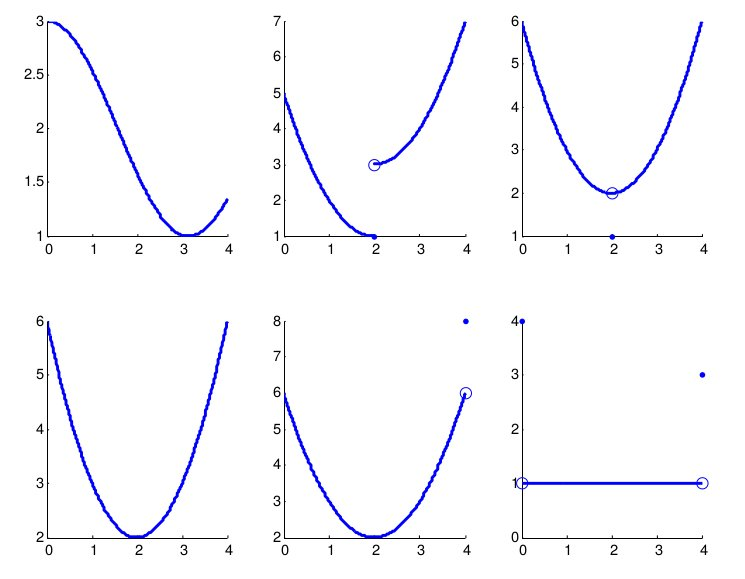
\includegraphics[scale=0.3]{conv_cont}\caption{Convex functions are continuous on interiors of convex sets.\label{fig:Convex-functions-are}}

\par\end{centering}

\end{figure}

\begin{defn*}
Let $S$ be a nonempty convex set in $\mathbb{R}^{n}$ and $f:S\rightarrow\mathbb{R}$
a convex function. Then $\xi$ is a \emph{subgradient} of $f$ at
$\bar{x}$ if
\[
f\left(x\right)\geq f\left(\bar{x}\right)+\xi^{t}\left(x-\bar{x}\right)
\]
I.e. $f\left(x\right)$ is above the plane defined by $f\left(\bar{x}\right)+\xi^{t}\left(x-\bar{x}\right)$.
$\xi$ is the \textbf{slope of the line or the gradient}.
\end{defn*}

\begin{defn*}
The set of all subgradients $\partial f\left(\bar{x}\right)$ of $f$
at $\bar{x}$ is called the \emph{subdifferential} of $f$ at $\bar{x}$.\end{defn*}
\begin{thm*}
Let $S$ be a nonempty convex set in $\mathbb{R}^{n}$ and $f:S\rightarrow\mathbb{R}$
a convex function. Then $f$ has a subgradient $\xi$ at $\bar{x}\in\text{int}\left(S\right)$.
In particular, the hyperplane 
\[
\mathcal{H}=\left\{ \left(x,y\right)\big|y=f\left(\bar{x}\right)+\xi^{t}\left(x-\bar{x}\right)\right\} 
\]
supports $\text{epi}\left(f\right)$ at $\left(\bar{x},f\left(\bar{x}\right)\right)$.\end{thm*}
\begin{proof}
Note that $\text{epi}\left(f\right)$ is convex and $\left(\bar{x},f\left(\bar{x}\right)\right)$
belongs to its boundary. Therefore by separation theorem there exists
$\left(\xi_{0},\mu\right)\in\mathbb{R}^{n}\times\mathbb{R}$. For
all $\left(\mathbf{x},y\right)\in\text{epi}\left(f\right)$. 
\[
\xi_{0}^{t}\left(x-\bar{x}\right)+\mu\left(y-f\left(\bar{x}\right)\right)\leq0
\]


Note that $\mu\leq0$ because otherwise take $y$ large enough and
the inequality would be violated. In fact $\mu<0$:
\begin{proof}
Toward a contradiction suppose $\mu=0$. Then $\xi_{0}^{t}\left(x-\bar{x}\right)\leq0$
for all $x\in S$. Since $\bar{x}\in\text{int}\left(S\right)$ there
exists $\lambda>0$ such that $x=\bar{x}+\lambda\xi_{0}\in S$ and
hence $\lambda\xi_{0}^{t}\xi_{0}\leq0$. This implies that $\xi_{0}=0$
(otherwise how could $\lambda\xi_{0}^{t}\xi_{0}$ negative or equal
to zero with $\lambda$ strictly positive). But then $\left(\xi_{0},\mu\right)=0$
contradicting the separation theorem. Therefore $\mu<0$.
\end{proof}
Dividing $\xi_{0}^{t}\left(x-\bar{x}\right)+\mu\left(y-f\left(\bar{x}\right)\right)\leq0$
by $\left|\mu\right|$
\[
\xi^{t}\left(x-\bar{x}\right)+-1\left(y-f\left(\bar{x}\right)\right)=\xi^{t}\left(x-\bar{x}\right)-y+f\left(\bar{x}\right)\leq0
\]
for all $\left(x,y\right)\in\text{epi}\left(f\right)$. Then by letting
$y\rightarrow f\left(x\right)$ we satisfy the theorem
\[
\xi^{t}\left(x-\bar{x}\right)+f\left(\bar{x}\right)\leq f\left(x\right)
\]
In particular, the hyperplane $H=\left\{ \left(x,y\right)\big|y=f\left(\bar{x}\right)+\xi^{t}\left(x-\bar{x}\right)\right\} $
supports $\text{epi}\left(f\right)$ at $\left(\bar{x},f\left(\bar{x}\right)\right)$.\end{proof}
\begin{cor*}
Let $S$ be a nonempty convex set in $\mathbb{R}^{n}$ and $f:S\rightarrow\mathbb{R}$
a strictly convex function. Then for $\bar{x}\in\text{int}\left(S\right)$,
there exists a vector $\xi$ such that 
\[
f\left(x\right)>f\left(\bar{x}\right)+\xi^{t}\left(x-\bar{x}\right)
\]
\end{cor*}
\begin{thm*}
Partial converse: let $S$ be a nonempty convex set in $\mathbb{R}^{n}$
and $f:S\rightarrow\mathbb{R}$. Suppose for each $\bar{x}\in\text{int}\left(S\right)$
there exists $\xi$
\[
f\left(x\right)\geq f\left(\bar{x}\right)+\xi^{t}\left(x-\bar{x}\right)
\]
for all $x\in S$. Then $f$ is convex on $\text{int}\left(S\right)$.\end{thm*}
\begin{defn*}
The \emph{directional derivative} is 
\[
f'\left(\bar{x},d\right)=\lim_{\lambda\rightarrow0^{+}}\frac{f\left(\bar{x}+\lambda d\right)-f\left(\bar{x}\right)}{\lambda}
\]
Alternatively it's $d\cdot\nabla f\left(\bar{x}\right)$\end{defn*}
\begin{thm*}
Let $f:\mathbb{R}^{n}\rightarrow\mathbb{R}$ be a convex function.
Then $f$ has all directional derivatives.\end{thm*}
\begin{proof}
Let $\lambda_{2}>\lambda_{1}>0$. By convexity of $f$ we have
\begin{align*}
f\left(\bar{x}+\lambda d\right) & =f\left(\frac{\lambda_{1}}{\lambda_{2}}\left(\bar{x}+\lambda_{2}d\right)+\left(1-\frac{\lambda_{1}}{\lambda_{2}}\right)\bar{x}\right)\\
 & \leq\frac{\lambda_{1}}{\lambda_{2}}f\left(\bar{x}+\lambda_{2}d\right)+\left(1-\frac{\lambda_{1}}{\lambda_{2}}\right)f\left(\bar{x}\right)
\end{align*}
which implies
\[
\frac{f\left(\bar{x}+\lambda_{1}d\right)-f\left(\bar{x}\right)}{\lambda_{1}}\leq\frac{f\left(\bar{x}+\lambda_{2}d\right)-f\left(\bar{x}\right)}{\lambda_{2}}
\]
Thus the difference quotient is monotonically decreasing. Then since
the function is convex it has a subgradient at $\bar{x}$ and so bounded
below. Therefore the limit converges.\end{proof}
\begin{defn*}
A function is called differentiable if there exists $v$ such that
\[
f\left(x\right)=f\left(\bar{x}\right)+v^{t}\left(x-\bar{x}\right)+\alpha\left(\bar{x},x-\bar{x}\right)\left\Vert x-\bar{x}\right\Vert 
\]
The function $\alpha$ is the Lagrange form of the first order remainder
term in the Taylor series approximation of $f$, i.e.
\[
\alpha\left(\bar{x},x-\bar{x}\right)\left\Vert x-\bar{x}\right\Vert =\frac{f^{''}\left(\bar{x}\right)}{3!}\left(x-\bar{x}\right)^{2}
\]

\end{defn*}
$v$ is called the gradient and duh is $\nabla f\left(\bar{x}\right)=\left(\frac{\partial f\left(\bar{x}\right)}{\partial x_{1}},\dots,\frac{\partial f\left(\bar{x}\right)}{\partial x_{n}}\right)$.
\begin{lem*}
Let $S$ be a nonempty convex set in $\mathbb{R}^{n}$ and $f:S\rightarrow\mathbb{R}$
a convex function and differentiable at $\bar{x}$. Then the subdifferential
at $\bar{x}$ is the singleton $\left\{ \nabla f\left(\bar{x}\right)\right\} $.\end{lem*}
\begin{proof}
Since $f$ is a convex set the subdifferential at $\bar{x}$ is not
empty. Let $\xi$ be a subgradient of $f$ at $\bar{x}$. Again by
the same theorem (existence of subgradients)
\[
f\left(\bar{x}+\lambda d\right)\geq f\left(\bar{x}\right)+\xi^{t}\left(\lambda d\right)
\]


By differentiability at $\bar{x}$
\[
f\left(\bar{x}+\lambda d\right)=f\left(\bar{x}\right)+\left(\nabla f\left(\bar{x}\right)\right)^{t}\left(\lambda d\right)+\alpha\left(\bar{x},\lambda d\right)\left\Vert \lambda d\right\Vert 
\]
Subtracting the equation from the inequality we get that 
\[
0\geq\xi^{t}\left(\lambda d\right)-\left(\nabla f\left(\bar{x}\right)\right)^{t}\left(\lambda d\right)-\alpha\left(\bar{x},\lambda d\right)\left\Vert \lambda d\right\Vert 
\]
Dividing by $\lambda$ and letting $\lambda\rightarrow0^{+}$ we get
that $\left(\xi-\nabla f\left(\bar{x}\right)\right)^{t}d\leq0$. Since
this is true for all $d$, choosing $d=\xi-\nabla f\left(\bar{x}\right)$
proves that $\xi-\nabla f\left(\bar{x}\right)=0$ (how else would
the norm squared of it be nonpositive).
\end{proof}
In light of the lemma, and supporting hyperplane, and the partial
converse we have another characterization of convex functions:
\begin{thm*}
Let $S$ be a nonempty open (or $\bar{x}\in\text{int}\left(S\right)$)
convex set in $\mathbb{R}^{n}$ and $f:S\rightarrow\mathbb{R}$ differentiable.
Then $f$ is convex iff $\forall\bar{x}\in S$
\[
f\left(x\right)\geq f\left(\bar{x}\right)+\left(\nabla f\left(\bar{x}\right)\right)^{t}\left(x-\bar{x}\right)
\]

\end{thm*}

\begin{thm*}
Let $S$ be a nonempty open (or $\bar{x}\in\text{int}\left(S\right)$)
convex set in $\mathbb{R}^{n}$ and $f:S\rightarrow\mathbb{R}$ differentiable.
Then $f$ is convex iff $\forall x_{1},x_{2}\in S$
\[
\left(\nabla f\left(x_{2}\right)-\nabla f\left(x_{1}\right)\right)^{t}\left(x_{2}-x_{1}\right)\geq0
\]
\end{thm*}
\begin{proof}
By characterization of convexity we have that 
\begin{align*}
f\left(x_{1}\right) & \geq f\left(x_{2}\right)+\left(\nabla f\left(x_{2}\right)\right)^{t}\left(x_{1}-x_{2}\right)\\
f\left(x_{2}\right) & \geq f\left(x_{1}\right)+\left(\nabla f\left(x_{1}\right)\right)^{t}\left(x_{2}-x_{1}\right)
\end{align*}
Adding the two inequalities gets the result. To prove the converse
use the mean value theorem:
\[
f\left(x_{2}\right)-f\left(x_{1}\right)=\left(\nabla f\left(x\right)\right)^{t}\left(x_{2}-x_{1}\right)
\]
where $x=\lambda x_{1}+\left(1-\lambda\right)x_{2}$ for $\lambda\in\left(0,1\right)$.
By assumption $\left(\nabla f\left(x\right)-\nabla f\left(x_{1}\right)\right)^{t}\left(x-x_{1}\right)\geq0$
which is equivalent to 
\[
\left(1-\lambda\right)\left(\nabla f\left(x\right)-\nabla f\left(x_{1}\right)\right)^{t}\left(x_{2}-x_{1}\right)\geq0
\]
This implies that 
\[
\left(\nabla f\left(x\right)\right)^{t}\left(x_{2}-x_{1}\right)\geq\left(\nabla f\left(x_{1}\right)\right)^{t}\left(x_{2}-x_{1}\right)
\]
But by mean value theorem result we get that 
\[
f\left(x_{2}\right)-f\left(x_{1}\right)\geq\left(\nabla f\left(x_{1}\right)\right)^{t}\left(x_{2}-x_{1}\right)
\]
and so by previous characterization we get that $f$ is convex.
\end{proof}
This is a first order condition on convexity. How about second order
conditions?
\begin{defn*}
A function $f$ is twice differentiable if 
\[
f\left(x\right)=f\left(\bar{x}\right)+\nabla f\left(\bar{x}\right)^{t}\left(x-\bar{x}\right)+\frac{1}{2}\left(x-\bar{x}\right)^{t}H\left(\bar{x}\right)\left(x-\bar{x}\right)+\alpha\left(\bar{x},x-\bar{x}\right)\left\Vert x-\bar{x}\right\Vert ^{2}
\]
and $\lim_{x\rightarrow\bar{x}}\alpha\left(\bar{x},x-\bar{x}\right)=0$.\end{defn*}
\begin{thm*}
Let $S$ be a nonempty open (or $\bar{x}\in\text{int}\left(S\right)$)
convex set in $\mathbb{R}^{n}$ and $f:S\rightarrow\mathbb{R}$ twice
differentiable. Then $f$ is convex iff $\nabla^{2}f\left(\bar{x}\right)$
is psd.
\end{thm*}
For strict convexity you need something stronger.
\begin{thm*}
Let $S$ be a nonempty open (or $\bar{x}\in\text{int}\left(S\right)$)
convex set in $\mathbb{R}^{n}$ and $f:S\rightarrow\mathbb{R}$ twice
differentiable. Then 
\begin{enumerate}
\item $\nabla^{2}f\left(\bar{x}\right)$ is pd then $f$ is strictly convex.
\item f is strictly convex then $\nabla^{2}f\left(\bar{x}\right)$ is psd.
\item f is strictly convex and quadratic then $\nabla^{2}f\left(\bar{x}\right)$
is pd.
\end{enumerate}
\end{thm*}

\section{Optimality conditions for Convex programs}
\begin{defn*}
Consider 
\begin{align*}
\min_{x} & f\left(x\right)\\
\text{s.t.} & x\in S
\end{align*}

\begin{enumerate}
\item $\bar{x}\in S$ is a \textbf{feasible solution} to the problem.
\item $\bar{x}\in S$ such that $f\left(\bar{x}\right)\leq f\left(x\right)$
for all $x\in S$ is a \textbf{globally optimal solution}.
\item $\bar{x}\in S$ such that $f\left(\bar{x}\right)\leq f\left(x\right)$
for all $x\in S\cap\mathcal{N}_{\epsilon}\left(\bar{x}\right)$, i.e.
in some neighborhood of $\bar{x}$ is a \textbf{locally optimal} \textbf{solution}.
\item $\bar{x}\in S$ such that $f\left(\bar{x}\right)<f\left(x\right)$
for all $x\in S\cap\mathcal{N}_{\epsilon}\left(\bar{x}\right)$, i.e.
in some neighborhood of $\bar{x}$ is a \textbf{strict locally optimal}
\textbf{solution}.
\item $\bar{x}\in S$ such that $f\left(\bar{x}\right)<f\left(x\right)$
for all $x\in S\cap\mathcal{N}_{\epsilon}\left(\bar{x}\right)$, i.e.
in some neighborhood of $\bar{x}$ and $\bar{x}$ is the only such
point is an \textbf{isolated locally optimal} \textbf{solution}.
\end{enumerate}
\end{defn*}
\begin{figure}[H]


\noindent \begin{centering}
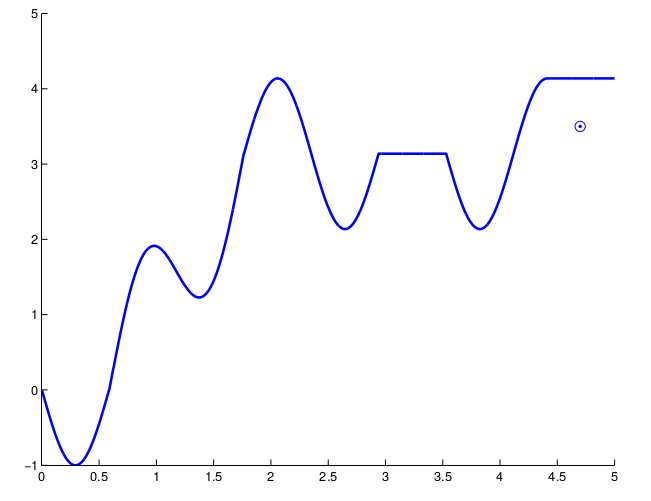
\includegraphics[scale=0.5]{solns}\caption{Characterizing solutions}

\par\end{centering}

\end{figure}

\begin{thm*}
Let $S$ be a nonempty convex set in $\mathbb{R}^{n}$ and $f:S\rightarrow\mathbb{R}$
convex and $\bar{x}$ be a locally optimal solution (optimal, but
not uniquely, within an $\epsilon$-ball) to $\min_{x\in S}f\left(x\right)$.
Then
\begin{enumerate}
\item $\bar{x}$ is globally optimal.
\item If $\bar{x}$ is strictly locally optimal ($f\left(\bar{x}\right)<f\left(x\right)$
in the $\epsilon$-ball). or $f$ is strictly convex then

\begin{enumerate}
\item $\bar{x}$ is uniquely globally optimal.
\item $\bar{x}$ is strongly (isolated) locally optimal.
\end{enumerate}
\end{enumerate}
\end{thm*}
\begin{proof}
Towards a contradiction suppose $\bar{x}$ is not globally optimal.
Note $\bar{x}$ locally optimal means $f\left(\bar{x}\right)\leq f\left(x\right)$
for $x\in S\cap\mathcal{N}_{\epsilon}\left(\bar{x}\right)$ with $\epsilon>0$.
Then not being global means there exists $\hat{x}$ such that $f\left(\hat{x}\right)<f\left(\bar{x}\right)$.
By convexity of $f$ 
\[
f\left(\lambda\hat{x}+\left(1-\lambda\right)\bar{x}\right)\leq\lambda f\left(\hat{x}\right)+\left(1-\lambda\right)f\left(\bar{x}\right)
\]
Then using $f\left(\hat{x}\right)<f\left(\bar{x}\right)$
\[
f\left(\lambda\hat{x}+\left(1-\lambda\right)\bar{x}\right)\leq\lambda f\left(\hat{x}\right)+\left(1-\lambda\right)f\left(\bar{x}\right)<\lambda f\left(\bar{x}\right)+\left(1-\lambda\right)f\left(\bar{x}\right)=f\left(\bar{x}\right)
\]
Taking $\lambda<\epsilon$ we get a contradiction. That handles part
1.

Part 2(a): Suppose $\bar{x}$ is a strict local optimal. Then by part
1 it's a global optimum. Suppose there exists $\hat{x}$ such that
$f\left(\bar{x}\right)=f\left(\hat{x}\right)$. Then 
\[
f\left(x_{\lambda}\right)=f\left(\lambda\hat{x}+\left(1-\lambda\right)\bar{x}\right)\leq\lambda f\left(\hat{x}\right)+\left(1-\lambda\right)f\left(\bar{x}\right)=\lambda f\left(\bar{x}\right)+\left(1-\lambda\right)f\left(\bar{x}\right)=f\left(\bar{x}\right)
\]
and by taking $\lambda<\epsilon$ we get a contradiction to strict
local optimality. Hence $\bar{x}$ is the unique global minimum. 

Part 2(b): Since it's a unique global minimum it must be isolated
since any other local minimum $\bar{x}$ in $S\cap\mathcal{N}_{\epsilon}\left(\bar{x}\right)$
would be a global minimum.

Part 2'(a/b): Suppose $\bar{x}$ is a local optimum and $f$ is strictly
convex. Since strictly convex implies convexity $\bar{x}$ is still
a global minimum. Towards a contradiction suppose $\bar{x}$ is not
unique, i.e. there exists $\hat{x}$ such that $f\left(\hat{x}\right)=f\left(\bar{x}\right)$.
By strict convexity
\[
f\left(\frac{\bar{x}+\hat{x}}{2}\right)<\frac{1}{2}f\left(\bar{x}\right)+\frac{1}{2}f\left(\hat{x}\right)=f\left(\bar{x}\right)
\]
By convexity of $S$ we have $\frac{\bar{x}+\hat{x}}{2}\in S$ and
therefore a contradiction of global optimality. Further similarly
$\bar{x}$ is also isolated.\end{proof}
\begin{thm*}
Let $f:\mathbb{R}^{n}\rightarrow\mathbb{R}$ be a convex function
and $S\neq\emptyset$ a convex subset of $\mathbb{R}^{n}$ and $\bar{x}\in S$.
Then for 
\[
\min_{x\in S}\,f\left(x\right)
\]
$\bar{x}$ is globally optimal iff $f$ has a supporting subgradient
$\xi$ such that $\xi^{t}\left(x-\bar{x}\right)\geq0$ for all $x\in S$.\end{thm*}
\begin{proof}
$\Leftarrow$ Suppose there exists $\xi$ such that $\xi^{t}\left(x-\bar{x}\right)\geq0$
for all $x\in S$. By convexity of $f$ 
\[
f\left(x\right)\geq f\left(\bar{x}\right)+\xi^{t}\left(x-\bar{x}\right)\geq f\left(\bar{x}\right)
\]
since $\xi^{t}\left(x-\bar{x}\right)$. Hence $\bar{x}$ is optimal.

$\Rightarrow$ Suppose $\bar{x}$ is optimal. Let 
\begin{align*}
\Lambda_{1} & =\left\{ \left(x-\bar{x},y\right)\big|x\in\mathbb{R}^{n},y>f\left(x\right)-f\left(\bar{x}\right)\right\} \\
\Lambda_{2} & =\left\{ \left(x-\bar{x},y\right)\big|x\in S,y\leq0\right\} 
\end{align*}
Note that $\Lambda_{1}$ is the ``shifted'' epigraph of $f$, shifted
such that $\left(\bar{x},f\left(\bar{x}\right)\right)=\left(0,0\right)$.
Both $\Lambda_{1}$ and $\Lambda_{2}$ are convex. Also $\Lambda_{1}\cap\Lambda_{2}=\emptyset$
since otherwise there exists $\left(x,y\right)$ such that $x\in S$
and $0>y>f\left(x\right)-f\left(\bar{x}\right)$ contradicting $\bar{x}$
is optimal (since $0>f\left(x\right)-f\left(\bar{x}\right)\iff f\left(\bar{x}\right)>f\left(x\right)$).
By separating hyperplane theorem there exists a hyperplane that separates:
there exists nonzero $\left(\xi_{0},\mu\right)$ and $\alpha\neq0$
such that 
\begin{align*}
\xi_{0}^{t}\left(x-\bar{x}\right)+\mu y & \leq\alpha,\,\forall x\in\mathbb{R}^{n},\,y>f\left(x\right)-f\left(\bar{x}\right)\\
\xi_{0}^{t}\left(x-\bar{x}\right)+\mu y & \geq\alpha,\,\forall x\in S,\,y\leq0
\end{align*}
Then letting $x=\bar{x}$ and $y=0$ in the second inequality you
get that $\alpha\leq0$. Now letting $x=\bar{x}$ and $y=\epsilon>0$
in the first inequality and you get $\mu\epsilon\leq\alpha$. Since
this is true for every $\epsilon>0$ it's the case that $\alpha\geq0$
and therefore$\mu\leq0$. Therefore $\mu\leq0$ and $\alpha=0$. So
summarizing 
\begin{align*}
\xi_{0}^{t}\left(x-\bar{x}\right)+\mu y & \leq0,\,\forall x\in\mathbb{R}^{n},\,y>f\left(x\right)-f\left(\bar{x}\right)\\
\xi_{0}^{t}\left(x-\bar{x}\right)+\mu y & \geq0,\,\forall x\in S,\,y\leq0
\end{align*}
If $\mu$ were 0 then $\xi_{0}^{t}\left(x-\bar{x}\right)\leq0$ for
all $x\in\mathbb{R}^{n}$ and then letting $x=\bar{x}+\xi_{0}$ shows
that $\xi_{0}=0$ which isn't possible. So $\mu<0$. Dividing by $\left|\mu\right|$
everywhere we get that 
\begin{align*}
\xi^{t}\left(x-\bar{x}\right)-y & \leq0,\,\forall x\in\mathbb{R}^{n},\,y>f\left(x\right)-f\left(\bar{x}\right)\\
\xi^{t}\left(x-\bar{x}\right)-y & \geq0,\,\forall x\in S,\,y\leq0
\end{align*}
Letting $y=0$ in the second inequality we get that $\xi^{t}\left(x-\bar{x}\right)\geq0$
for all $x\in S$. From the first inequality we conclude that since
$\xi^{t}\left(x-\bar{x}\right)-y\leq0$ for all $\left(x,y\right)$
in the ``shifted'' strict epigraph of $f$ it must therefore also
hold in the closure, i.e. where $y=f\left(x\right)-f\left(\bar{x}\right)$,
which gives us
\[
f\left(x\right)\geq f\left(\bar{x}\right)+\xi^{t}\left(x-\bar{x}\right)
\]
\end{proof}
\begin{cor*}
If $S$ is open then $\bar{x}$ is global optimal iff $0\in\partial f\left(\bar{x}\right)$\end{cor*}
\begin{proof}
$\bar{x}$ is optimal iff there exists $\xi$ such that $\xi^{t}\left(x-\bar{x}\right)\geq0$.
Since $S$ is open take $\lambda$ such that $x=\bar{x}-\lambda\xi\in S$
and then 
\[
-\lambda\left\Vert \xi\right\Vert ^{2}\geq0
\]

\end{proof}

\begin{cor*}
If $f$ differentiable (and convex) then
\begin{enumerate}
\item $\bar{x}$ is globally optimal iff $\nabla f\left(\bar{x}\right)^{t}\left(x-\bar{x}\right)\geq0$
\item If $S$ is open then $\bar{x}$ is globally optimal iff $\nabla f\left(\bar{x}\right)=0$
\end{enumerate}
\end{cor*}
\begin{proof}
Obvious since $\partial f\left(\bar{x}\right)=\left\{ \nabla f\left(\bar{x}\right)\right\} $.
\end{proof}
\begin{figure}[H]


\noindent \begin{centering}
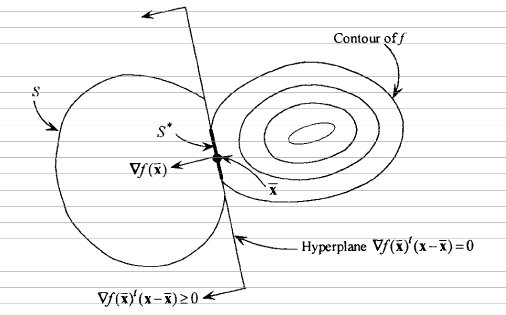
\includegraphics[scale=0.5]{grad_dir}\caption{Gradient angle\label{fig:Gradient-angle}}

\par\end{centering}

\end{figure}


Consider figure \ref{fig:Gradient-angle}. Suppose the problem is
to minimize $f$ subject to $x\in S$ and $f$ is differentiable and
convex but $S$ is arbitrary. Suppose at some $\bar{x}$ the directional
derivative $\nabla f\left(\bar{x}\right)\left(x-\bar{x}\right)\geq0$
for all $x\in S$. Then going in any direction in $S$ would potentially
increase the objective, regardless of what $S$ is like. Why? By convexity\footnote{At every $\bar{x}$ we have that $f\left(x\right)\geq f\left(\bar{x}\right)+\nabla f\left(\bar{x}\right)^{t}\left(x-\bar{x}\right)$. }and
differentiability of $f$ any solution $\hat{x}$ (anywhere in $\mathbb{R}^{n}$,
which is a convex set) that improves on $\bar{x}$
\[
f\left(\bar{x}\right)>f\left(\hat{x}\right)\geq f\left(\bar{x}\right)+\nabla f\left(\bar{x}\right)^{t}\left(\hat{x}-\bar{x}\right)
\]
which implies $\nabla f\left(\bar{x}\right)^{t}\left(\hat{x}-\bar{x}\right)<f\left(\bar{x}\right)-f\left(\bar{x}\right)=0$
but $\nabla f\left(\bar{x}\right)^{t}\left(x-\bar{x}\right)\geq0$
for all $x\in S$. Hence the hyperplane $\nabla f\left(\bar{x}\right)^{t}\left(\hat{x}-\bar{x}\right)=0$
separates $S$ (arbitrary $S$) from solutions that improve cost.
In the non-differentiable case the supporting hyperplane $\xi$ plays
the same role as $\nabla f\left(\bar{x}\right)$. Conversely suppose
$f$ is differentiable but arbitrary otherwise and $S$ is convex.
Then $\bar{x}$ is a global minimum then again $\nabla f\left(\bar{x}\right)\left(x-\bar{x}\right)\geq0$
since otherwise if there exists $x\in\text{int}\left(S\right)$ such
that $\nabla f\left(\bar{x}\right)^{t}\left(x-\bar{x}\right)<0$ you
could do go in the direction $d=x-\bar{x}$, improve cost, and still
satisfy constraints. The general take away is: if $f$ is differentiable
and otherwise $f$ and $S$ are arbitrary and $\bar{x}$ is a local
minimum then for any feasible direction $d$ such that $x=\bar{x}+\lambda d$
it must be the case that 
\[
\nabla f\left(\bar{x}\right)^{t}d\geq0
\]
for some $0<\lambda\leq\delta$ i.e. going in that direction for a
small enough step does not improve the objective. 

Back to your original program:

What characterizes the set of optimal solutions to $\min\left\{ f\left(x\right)\big|x\in S\right\} $
when $f$ is convex and differentiable and so is $S$? 
\begin{thm*}
If $f$ is convex and differentiable and $S$ is convex. Suppose there
exists an optimal solution $\bar{x}$. Then the set of optimal solution
$S^{*}$
\[
S^{*}=\left\{ x\in S\big|\nabla f\left(\bar{x}\right)^{t}\left(x-\bar{x}\right)\leq0,\nabla f\left(x\right)=\nabla f\left(\bar{x}\right)\right\} 
\]
\end{thm*}
\begin{proof}
Denote the candidate set of optimal solutions by $\bar{S}$ and note
that $\bar{x}\in\bar{S}$. Consider $\hat{x}\in S^{*}$. By convexity
of $f$ (and convexity of $S$) and definition of $S^{*}$, it's the
case that $\hat{x}\in S$
\[
f\left(\bar{x}\right)\geq f\left(\hat{x}\right)+\nabla f\left(\hat{x}\right)^{t}\left(\bar{x}-\hat{x}\right)=f\left(\hat{x}\right)+\nabla f\left(\bar{x}\right)^{t}\left(\bar{x}-\hat{x}\right)=f\left(\hat{x}\right)+\left(-\nabla f\left(\bar{x}\right)^{t}\left(\hat{x}-\bar{x}\right)\right)\geq f\left(\hat{x}\right)
\]
Hence $\hat{x}\in\bar{S}$ and so $S^{*}\subset\bar{S}$. Conversely,
suppose $\hat{x}\in\bar{S}$ then $f\left(\hat{x}\right)=f\left(\bar{x}\right)$
and so
\[
f\left(\bar{x}\right)=f\left(\hat{x}\right)\geq f\left(\bar{x}\right)+\nabla f\left(\bar{x}\right)^{t}\left(\hat{x}-\bar{x}\right)
\]
and hence $\nabla f\left(\bar{x}\right)^{t}\left(\hat{x}-\bar{x}\right)\leq0$
but by corollary above $\nabla f\left(\bar{x}\right)^{t}\left(\hat{x}-\bar{x}\right)\geq0$
and hence $\nabla f\left(\bar{x}\right)^{t}\left(\hat{x}-\bar{x}\right)=0$.
Interchanging $\hat{x}$ and $\bar{x}$ we get that $\nabla f\left(\bar{x}\right)^{t}\left(\bar{x}-\hat{x}\right)=0$
and subtracting we get
\[
\left(\nabla f\left(\bar{x}\right)-\nabla f\left(\hat{x}\right)\right)^{t}\left(\bar{x}-\hat{x}\right)=0
\]
But 
\begin{align*}
\left(\nabla f\left(\bar{x}\right)-\nabla f\left(\hat{x}\right)\right) & =\left.\nabla f\left(\hat{x}+\lambda\left(\bar{x}-\hat{x}\right)\right)\right|_{\lambda=0}^{\lambda=1}\\
 & =\int_{0}^{1}\nabla^{2}f\left(\hat{x}+\lambda\left(\bar{x}-\hat{x}\right)\right)\left(\bar{x}-\hat{x}\right)d\lambda\eqqcolon G\left(\bar{x}-\hat{x}\right)
\end{align*}
Note that $G$ is psd since $\nabla^{2}f$ is psd (since $f$ is convex).
Then 
\[
0=\left(\bar{x}-\hat{x}\right)^{t}\left(\nabla f\left(\bar{x}\right)-\nabla f\left(\hat{x}\right)\right)=\left(\bar{x}-\hat{x}\right)^{t}G\left(\bar{x}-\hat{x}\right)
\]
and by psd-ness $G\left(\bar{x}-\hat{x}\right)$ must be 0 and hence
$\nabla f\left(\bar{x}\right)-\nabla f\left(\hat{x}\right)=0$ (and
$\nabla f\left(\bar{x}\right)^{t}\left(\hat{x}-\bar{x}\right)\leq0$)
and hence $\hat{x}\in S^{*}$ and so $\bar{S}\subset S^{*}$.\end{proof}
\begin{cor*}
The set of alternative solutions $S^{*}$ for convex, twice differentiable,
and convex $S$ can be characterized as
\[
S^{*}=\left\{ x\in S\big|\nabla f\left(\bar{x}\right)^{t}\left(x-\bar{x}\right)=0,\nabla f\left(x\right)=\nabla f\left(\bar{x}\right)\right\} 
\]
\end{cor*}
\begin{proof}
Follows from previous theorem and for optimal $\bar{x}$, and all
other $x\in S$, $\nabla f\left(\bar{x}\right)\left(x-\bar{x}\right)\geq0$.\end{proof}
\begin{cor*}
Suppose $f=c^{t}x+\frac{1}{2}x^{t}Hx$ and $S$ is polyhedral. Then
$S^{*}$ is the polyhedral set given by
\[
S^{*}=\left\{ x\in S\big|c^{t}\left(x-\bar{x}\right)=0,H\left(x-\bar{x}\right)=0\right\} 
\]
\end{cor*}
\begin{proof}
$\nabla f\left(x\right)=c+Hx$
\end{proof}
For maxima of convex functions similar things apply (but for different
reasons). 
\begin{thm*}
If $f$ is convex and $S$ a nonempty convex set, if $\bar{x}$ is
a local optimal then for all $\xi$ it's the case that $\xi^{t}\left(x-\bar{x}\right)\leq0$
for each $x\in S$.\end{thm*}
\begin{proof}
Suppose $\bar{x}\in S$ is a local optimum. Then for all $x\in S\cap\mathcal{N}_{\epsilon}\left(\bar{x}\right)$
it's the case that $f\left(x\right)\leq f\left(\bar{x}\right)$. Let
$\lambda<\epsilon$ and then
\[
f\left(\bar{x}+\lambda\left(x-\bar{x}\right)\right)\le f\left(\bar{x}\right)
\]
Then by convexity of $f$ for all $\xi$
\[
f\left(\bar{x}+\lambda\left(x-\bar{x}\right)\right)\geq f\left(\bar{x}\right)+\lambda\xi^{t}\left(x-\bar{x}\right)
\]
implying $\lambda\xi^{t}\left(x-\bar{x}\right)\leq0$. Divinding by
$\lambda$ we have it.\end{proof}
\begin{cor*}
If $f$ is differentiable them $\nabla f\left(\bar{x}\right)\left(x-\bar{x}\right)\le0$. 
\end{cor*}
The result is necessary but not sufficient for gradients to be as
such.
\begin{thm*}
If $f$ is a convex function and $S$ a nonempty polyhedral set then
the solution to a maximization problem is at the boudary (i.e. extreme
point).\end{thm*}
\begin{proof}
Note $f$ is continuous because it's convex and $S$ is compact (bounded
over $\mathbb{R}^{n}$) and hence $f$ achieves its maximum at $x'\in S$.
By the representation theorem $S$ is defined only as a convex combination
of extreme points hence 
\[
x^{'}=\sum_{j=1}^{k}\lambda_{j}x_{j},\sum_{j=1}^{k}\lambda_{j}=1
\]
and $\lambda_{j}\geq0$ and $x_{j}$ are extreme points. By convexity
of $f$ 
\[
f\left(\sum_{j=1}^{k}\lambda_{j}x_{j}\right)\leq\sum_{j=1}^{k}\lambda_{j}f\left(x_{j}\right)
\]
But $f\left(x^{'}\right)\geq f\left(x_{j}\right)$ for all $j$ and
thus $f\left(x^{'}\right)=f\left(x_{j}\right)$. Therefore the solutions
are all at the bounday points.
\end{proof}

\section{Optimality conditions for unconstrained problems}
\begin{defn*}
Consider $\min_{x\in\mathbb{R}^{n}}f\left(x\right)$. Then $d$ is
an \emph{improving} direction at $\bar{x}$ if $f\left(\bar{x}+\lambda d\right)<f\left(\bar{x}\right)$
for $0<\lambda<\epsilon$ for some $\epsilon$. \end{defn*}
\begin{thm*}
Let $d$ be such that $\nabla f\left(\bar{x}\right)^{t}d<0$. Then
$d$ is an improving direction.\end{thm*}
\begin{proof}
Why? This says that going in the direction of is strictly acute with
$-\nabla f\left(\bar{x}\right)$, i.e. sort of aligned with the direction
of steepest descent. By differentiability of $f$ at $\bar{x}$ 
\[
f\left(\bar{x}+\lambda d\right)=f\left(\bar{x}\right)+\lambda\nabla f\left(\bar{x}\right)^{t}d+\lambda\left\Vert d\right\Vert \alpha\left(\bar{x},\lambda d\right)
\]
Re-arranging terms we get
\[
\frac{f\left(\bar{x}+\lambda d\right)-f\left(\bar{x}\right)}{\lambda}=\nabla f\left(\bar{x}\right)^{t}d+\left\Vert d\right\Vert \alpha\left(\bar{x},\lambda d\right)
\]
Since $\nabla f\left(\bar{x}\right)^{t}d<0$ and $\alpha\rightarrow0$
as $\lambda\rightarrow0$ there exists $\epsilon$ such that $\nabla f\left(\bar{x}\right)^{t}d+\left\Vert d\right\Vert \alpha\left(\bar{x},\lambda d\right)<0$
(we can make $\left\Vert d\right\Vert \alpha\left(\bar{x},\lambda d\right)$
smaller than $\nabla f\left(\bar{x}\right)^{t}d$) for all $0<\lambda<\epsilon$
and therefore 
\[
\frac{f\left(\bar{x}+\lambda d\right)-f\left(\bar{x}\right)}{\lambda}<0
\]
 and since $\lambda>0$ we have that $f\left(\bar{x}+\lambda d\right)-f\left(\bar{x}\right)<0$.\end{proof}
\begin{cor*}
If $\bar{x}$ is a local minimum then $\nabla f\left(\bar{x}\right)=0$.\end{cor*}
\begin{proof}
Towards a contradiction suppose $\nabla f\left(\bar{x}\right)\neq0$
and set $d=-\nabla f\left(\bar{x}\right)$. Then $\nabla f\left(\bar{x}\right)^{t}d=-\left\Vert \nabla f\left(\bar{x}\right)\right\Vert ^{2}<0$,
hence satisfying the previous result for this direction, hence $d$
is an improving direction contradicting that $\bar{x}$ is a local
minimum.
\end{proof}
\textbf{The converse is not true!}

Second order necessary conditions
\begin{thm*}
Let $f$ be twice differentiable at $\bar{x}$. If $\bar{x}$ is a
local minimum of $f$ then $\nabla f\left(\bar{x}\right)=0$ and $\nabla^{2}f\left(\bar{x}\right)$
is psd.\end{thm*}
\begin{proof}
First part follows from above. For the second part consider and arbitrary
direction 
\[
f\left(\bar{x}+\lambda d\right)=f\left(\bar{x}\right)+\lambda\nabla f\left(\bar{x}\right)^{t}d+\frac{1}{2}\lambda^{2}d^{t}H\left(\bar{x}\right)d+\lambda^{2}\left\Vert d\right\Vert ^{2}\alpha\left(\bar{x},\lambda d\right)
\]
Again $\nabla f\left(\bar{x}\right)=0$ and so
\[
\frac{f\left(\bar{x}+\lambda d\right)-f\left(\bar{x}\right)}{\lambda^{2}}=+\frac{1}{2}d^{t}H\left(\bar{x}\right)d+\left\Vert d\right\Vert ^{2}\alpha\left(\bar{x},\lambda d\right)
\]
Since $\bar{x}$ is local minimum $f\left(\bar{x}+\lambda d\right)-f\left(\bar{x}\right)\geq0$
for sufficiently small $\lambda$. Thus 
\[
\frac{1}{2}d^{t}H\left(\bar{x}\right)d+\left\Vert d\right\Vert ^{2}\alpha\left(\bar{x},\lambda d\right)\geq0
\]
Taking the limit as $\lambda\rightarrow0$ we get that $d^{t}H\left(\bar{x}\right)d\geq0$
for all directions $d$.
\end{proof}
\textbf{The converse is not true! But there is a partial converse}
\begin{thm*}
Let $f$ be twice differentiable at $\bar{x}$. If $\nabla f\left(\bar{x}\right)=0$
and $\nabla^{2}f\left(\bar{x}\right)$ pd then $\bar{x}$ is a strict
local minimum.\end{thm*}
\begin{proof}
Since $f$ is twice differentiable at $\bar{x}$ 
\[
f\left(\bar{x}+\lambda d\right)=f\left(\bar{x}\right)+\lambda\nabla f\left(\bar{x}\right)^{t}d+\frac{1}{2}\lambda^{2}d^{t}H\left(\bar{x}\right)d+\lambda^{2}\left\Vert d\right\Vert ^{2}\alpha\left(\bar{x},\lambda d\right)
\]
Towards a contradiction suppose $\bar{x}$ is not a strict local minimum.
We want find a direction along which $d^{t}Hd\leq0$. Since $\bar{x}$
is not a strict local minimum there exists a sequence $x_{k}$ such
that $f\left(x_{k}\right)\le f\left(\bar{x}\right)$. Denote 
\[
d_{k}=\frac{x_{k}-\bar{x}}{\left\Vert x_{k}-\bar{x}\right\Vert }
\]
and noting that $\nabla f\left(\bar{x}\right)=0$ we have that 
\[
\frac{1}{2}d_{k}^{t}H\left(\bar{x}\right)d+\alpha\left(\bar{x},x_{k}-\bar{x}\right)\leq0
\]
But $d_{k}$ is bounded (norm 1) and therefore there exists a subsequence
that converges to a direction $d$ such that $d^{t}Hd\leq0$.
\end{proof}
In certain instances we can say stronger things: 
\begin{thm*}
Let $f$ be \textbf{convex} and differentiable at $\bar{x}$. Then
$\bar{x}$ is a global minimum iff $\nabla f\left(\bar{x}\right)=0$\end{thm*}
\begin{proof}
By corollary to two theorems ago if global minimum then $\nabla f\left(\bar{x}\right)=0$.
For the converse suppose that $\nabla f\left(\bar{x}\right)=0$ so
that $\nabla f\left(\bar{x}\right)^{t}\left(x-\bar{x}\right)=0$.
By convexity 
\[
f\left(x\right)\geq f\left(\bar{x}\right)+\nabla f\left(\bar{x}\right)^{t}\left(x-\bar{x}\right)=f\left(\bar{x}\right)
\]

\end{proof}

\section{Optimality conditions for constrained problems}
\begin{defn*}
Let $S$ be a nonempty set in $\mathbb{R}^{n}$ and $\bar{x}\in\text{cl}\left(S\right)$.
The \textbf{\emph{cone of feasible directions}} of $S$ at $\bar{x}$,
denoted by $D$, is given by
\[
D=\left\{ d\big|\exists_{\delta}\forall_{0<\lambda<\delta}\,d\neq0,x+\lambda d\in S\right\} 
\]

\end{defn*}

\begin{defn*}
Given a function $f$ and a minimization problem the \textbf{\emph{cone
of improving directions }}at $\bar{x}$ is 
\[
F=\left\{ d\big|f\left(\bar{x}+\lambda\right)<f\left(\bar{x}\right)\text{ for all }\lambda\in\left(0,\delta\right)\text{ for some }\delta\right\} 
\]

\end{defn*}

\begin{defn*}
For differentiable $f$ at $\bar{x}$ a subset of the improving directions
(by theorem that says that $\nabla f\left(\bar{x}\right)^{t}d<0$
is an improving direction; $d$ makes a strictly acute angle with
$-\nabla f\left(\bar{x}\right)$ the direction of steepest descent)
is
\[
F_{0}=\left\{ d\big|\nabla f\left(\bar{x}\right)^{t}d<0\right\} 
\]
\end{defn*}
\begin{thm*}
For $\min\left\{ f\left(x\right)\big|x\in S\right\} $ with $f$ differentiable
at $\bar{x}\in S$. If $\bar{x}$ is a local optimal solution then
$F_{0}\cap D=\emptyset$.\end{thm*}
\begin{proof}
Towards a contradiction suppose $\bar{x}$ is locally optimal and
there exists $d\in F_{0}\cap D$. Then by improving direction theorem
($\nabla f\left(\bar{x}\right)^{t}d<0\Rightarrow\exists_{\delta>0}\forall_{\lambda\in\left(0,\delta\right)}\,f\left(\bar{x}+\lambda d\right)<f\left(\bar{x}\right)$)
there exists $\delta_{1}$ such that for all $\lambda\in\left(0,\delta_{1}\right)$
\[
f\left(\bar{x}+\lambda d\right)<f\left(\bar{x}\right)
\]
Then by definition of $D$ it's the case that there exists $\delta_{2}$
(possibly different from $\delta_{1}$) such that 
\[
\bar{x}+\lambda d\in S
\]
Taking $\delta=\min\left\{ \delta_{1},\delta_{2}\right\} $ and we
have that for $\lambda\in\left(0,\delta\right)$ it's the case that
$\bar{x}+\lambda d\in S$ and 
\[
f\left(\bar{x}+\lambda d\right)<f\left(\bar{x}\right)
\]


contradicting local optimality, a contradiction.
\end{proof}
There's a partial converse in the case of convex $f$
\begin{thm*}
Suppose $F_{0}\cap D=\emptyset$ and $f$ is convex at $\bar{x}$
and there exists a neighborhood $\mathcal{N}_{\epsilon}\left(\bar{x}\right)$
such that $\left(x-\bar{x}\right)\in D$ for any $x\in S\cap\mathcal{N}_{\epsilon}\left(\bar{x}\right)$
(i.e. feasible direction in the neighborhood). Then $\bar{x}$ is
a local minimum.\end{thm*}
\begin{proof}
Towards a contradiction suppose $F_{0}\cap D=\emptyset$ and $x-\bar{x}\in D$
for all $x\in\mathcal{N}_{\epsilon}\left(\bar{x}\right)\cap S$ and
there exists $\hat{x}$ such that $f\left(\hat{x}\right)<f\left(\bar{x}\right)$
for some $\hat{x}\in\mathcal{N}_{\epsilon}\left(\bar{x}\right)\cap S$,
i.e. $\bar{x}$ is not a local minimum. By assumption on $\mathcal{N}_{\epsilon}\left(\bar{x}\right)\cap S$
it's the case that $d=\hat{x}-\bar{x}\in D$. Furthermore by convexity
$\nabla f\left(\bar{x}\right)^{t}d<0$ (Suppose $\nabla f\left(\bar{x}\right)^{t}d\geq0$
we would have $f\left(\hat{x}\right)=f\left(\bar{x}+d\right)\geq f\left(\bar{x}\right)+\nabla f\left(\bar{x}\right)^{t}d\geq f\left(\bar{x}\right)$).
Therefore $d\in D$ and $d\in F_{0}$ which is a contradiction.
\end{proof}
The cone $F_{0}$ is an algebraic description of the set of improving
directions but $F_{0}\subset F$. There's another inclusion: if $d\in F$
then $\nabla f\left(\bar{x}\right)^{t}d\leq0$ (since $\nabla f\left(\bar{x}\right)^{t}d>0$
would make $d$ an ascent direction). Therefore
\[
F_{0}\subset F\subset F_{0}^{'}\coloneqq\left\{ d\neq0\big|\nabla f\left(\bar{x}\right)^{t}d\leq0\right\} 
\]


The unknown directions are those for which $\nabla f\left(\bar{x}\right)^{t}d=0$.
But in instances of convexity (concavity) we have tightness
\begin{thm*}
If $f$ is convex(concave) at $\bar{x}$ then $F=F_{0}$ ($F=F_{0}^{'}$).\end{thm*}
\begin{proof}
If $f$ is convex at $\bar{x}$ then if $\nabla f\left(\bar{x}\right)^{t}d\geq0$
it's the case that $f\left(\bar{x}+\lambda d\right)\geq f\left(\bar{x}\right)+\nabla f\left(\bar{x}\right)^{t}\left(\lambda d\right)\geq f\left(\bar{x}\right)$
for all $\lambda$. Recall that 
\[
F=\left\{ d\big|f\left(\bar{x}+\lambda\right)<f\left(\bar{x}\right)\text{ for all }\lambda\in\left(0,\delta\right)\text{ for some }\delta\right\} 
\]
and hence negating the above we get that $d\in F$ implies $d\in F_{0}$,
i.e. $F\subset F_{0}$ and so $F=F_{0}$. Now if $f$ is strictly
concave then we know that whenever $d\in F_{0}^{'}$ we have $f\left(\bar{x}+\lambda d\right)<f\left(\bar{x}\right)$
and therefore $F_{0}^{'}\subset F$ and hence $F=F_{0}^{'}$.\end{proof}
\begin{defn*}
From the improving directions theorem if $\nabla f\left(\bar{x}\right)^{t}d<0$
then $d$ is an improving direction ).
\end{defn*}
Specify the feasible region using functions $g_{i}$ now
\[
S=\left\{ x\in X\big|g_{i}\left(x\right)\leq0\right\} 
\]
We'd like to characterize $D$ algebraically so that we can establish
algebraic constraints on the objective and constraints for optimality.
\begin{lem*}
Let 
\[
S=\left\{ x\in X\big|g_{i}\left(x\right)\leq0,i\in M=\left\{ 1,\dots,m\right\} \right\} 
\]
Given a feasible $\bar{x}$ let $I\subset M$ be set of $i$ such
that $g_{i}\left(\bar{x}\right)=0$ (the set of binding constraints)
and assume $g_{I}$ are differentiable at $\bar{x}$ and $M-I$ are
continuous at $\bar{x}$. Define $G_{0}$ and $G_{0}^{'}$ analogously
to $F_{0}$ and $F_{0}^{'}$, i.e.
\begin{align*}
G_{0} & =\left\{ d\big|d\neq0,\nabla g_{i}\left(\bar{x}\right)^{t}d<0,i\in I\right\} \\
G_{0}^{'} & =\left\{ d\big|d\neq0,\nabla g_{i}\left(\bar{x}\right)^{t}d\leq0,i\in I\right\} 
\end{align*}
Then 
\[
G_{0}\subset D\subset G_{0}^{'}
\]
\end{lem*}
\begin{proof}
Let $d\in G_{0}$. Since $\bar{x}\in X$ and $X$ is open there exists
$\delta_{1}>0$ such that $\bar{x}+\lambda d\in X$ for $\lambda\in\left(0,\delta_{1}\right)$.
Also, since $g_{M-I}\left(\bar{x}\right)<0$ and $g_{M-I}$ are continuous
at $\bar{x}$ there exists $\delta_{2}>0$ such that 
\[
g_{M-I}\left(\bar{x}+\lambda d\right)<0\text{ for }\lambda\in\left(0,\delta_{2}\right)
\]
Furthermore since $d\in G_{0}$, $\nabla g_{I}\left(\bar{x}\right)^{t}d<0$
and so by the increasing direction theorem there exists $\delta_{3}>0$
such that 
\[
g_{I}\left(\bar{x}+\lambda d\right)<g_{I}\left(\bar{x}\right)=0\text{ for }\lambda\in\left(0,\delta_{3}\right)
\]
Let $\delta=\min\left\{ \delta_{1},\delta_{2},\delta_{3}\right\} >0$
and it's clear that $x=\bar{x}+\lambda d\in S$ for $\lambda\in\left(0,\delta\right)$
(why? all constraints are satisfied). Thus $d\in D$, where $D$ is
the cone of feasible directions of the feasible region at $\bar{x}$
. Thus $G_{0}\subset D$. Similarly if $d\in G_{0}^{'}$ if $\nabla g_{i}\left(\bar{x}\right)^{t}d>0$
for any $i\in I$ then $g_{i}\left(\bar{x}+\lambda d\right)>g_{i}\left(\bar{x}\right)=0$
for $\lambda$ sufficiently small, contradicting that $d\in D$, and
thus $D\subset G_{0}^{'}$.
\end{proof}
Finer results in the case of convexity/concavity
\begin{lem*}
If $g_{I}$ are strictly convex at $\bar{x}$ then $D=G_{0}$ and
if $g_{I}$ are concave then $D=G_{0}^{'}$.\end{lem*}
\begin{proof}
Suppose $g_{I}$ are strictly convex at $\bar{x}$ and let $d\in D$.
If $d\not\in G_{0}$ then $\nabla g_{i}\left(\bar{x}\right)^{t}d\geq0$
for some $i\in I$ we would have $g_{i}\left(\bar{x}+\lambda d\right)>g_{i}\left(\bar{x}\right)=0$
for all $\lambda>0$ condtradicting $d\in D$. Hence in this case
$D=G_{0}$. Now suppose $g_{I}$ are concave at $\bar{x}$ and let
$d\in G_{0}^{'}$. Then $g_{I}\left(\bar{x}+\lambda d\right)\leq g_{I}\left(\bar{x}\right)$
for all $\lambda\geq0$ and by continuity of $g_{M-I}$ and since
$X$ is open we obtain $\bar{x}+\lambda d\in S$ for all $\lambda$
sufficiently small and hence $d\in D$. Hence $G_{0}^{'}\subset D\subset G_{0}^{'}$.\end{proof}
\begin{thm*}
Consider
\[
\min\left\{ f\left(x\right)\big|g_{i}\left(x\right)\leq0,i\in M=\left\{ 1,\dots,m\right\} \right\} 
\]
Let $\bar{x}$ be feasible and $I$ as before. Assume that $f$ and
$g_{I}$ are differentiable at $\bar{x}$ and $g_{M-I}$ are continuous
at $\bar{x}$. Then
\begin{enumerate}
\item If $\bar{x}$ is locally optimal then $F_{0}\cap G_{0}=\emptyset$.
\item If $F_{0}\cap G_{0}=\emptyset$ and $f$ is convex, $g_{I}$ strictly
convex in some neighborhood of $\bar{x}$, then $\bar{x}$ is a local
minimum.
\end{enumerate}
\end{thm*}
\begin{proof}
Let $\bar{x}$ be locally optimal then $F_{0}\cap D=\emptyset$ by
two theorems above and by $G_{0}\subset D$ we have $F_{0}\cap G_{0}=\emptyset$.
Conversely suppose $F_{0}\cap G_{0}=\emptyset$ and $f,g_{i}$ are
as specified. Redefining the feasible region as those $x$ which satisfy
the binding constraints we have that $G_{0}=D$ by above lemma about
strict convexity and hence $F_{0}\cap D=\emptyset$. Further since
the level sets $g_{I}\left(x\right)\le0$ are convex over some $\mathcal{N}_{\epsilon}\left(\bar{x}\right)$
it follows that $S\cap N_{\epsilon}\left(\bar{x}\right)$ is convex
($S$ is the feasible region spanned by feasible directions). Since
$F_{0}\cap D=\emptyset$ and $f$ is convex at $\bar{x}$ from the
converse of improving directions set theorem that $\bar{x}$ is a
local minimum. Throwing the nonbinding constraints back in doesn't
change anything.
\end{proof}
Now to finally turn the geometric constraint $F_{0}\cap G_{0}=\emptyset$
into something useful:
\begin{thm*}
Fritz-John ``necessary'' conditions. Let $X$ be nonempty open.
Consider 
\[
\min\left\{ f\left(x\right)\big|x\in X,g_{i}\left(x\right)\leq0,i\in M=\left\{ 1,\dots,m\right\} \right\} 
\]
Let $\bar{x}$ be feasible and $g_{I}\left(\bar{x}\right)=0$. Furthermore
suppose that $f$ and $g_{I}$ are differentiable and $g_{M-I}$ are
continuous at $\bar{x}$. If $\bar{x}$ is locally optimal then there
exist Lagrange multipliers $u_{0},u_{I}$ such that
\begin{align*}
u_{0}\nabla f\left(\bar{x}\right)+\sum_{i=I}u_{i}\nabla g_{i}\left(\bar{x}\right) & =0\\
u_{0},u_{I} & \geq0\\
\left(u_{0},u_{I}\right) & \neq\left(0,0\right)
\end{align*}
Alternatively this can be rewritten as 
\begin{align*}
u_{0}\nabla f\left(\bar{x}\right)+\sum_{i=1}^{m}u_{i}\nabla g_{i}\left(\bar{x}\right) & =0\\
u_{I}g_{I}\left(\bar{x}\right) & =0\\
u_{0},u_{I} & \geq0\\
\left(u_{0},u\right) & \neq\left(0,0\right)
\end{align*}
\end{thm*}
\begin{proof}
Since $\bar{x}$ is locally optimal $F_{0}\cap G_{0}=\emptyset$,
i.e. there exists no $d$ such that $\nabla f\left(\bar{x}\right)^{t}d<0$
and $\nabla g_{I}\left(\bar{x}\right)^{t}d<0$. Let 
\[
\nabla L=\begin{bmatrix}\nabla f\left(\bar{x}\right)^{t}\\
\nabla g_{i}\left(\bar{x}\right)^{t}
\end{bmatrix}
\]
Then this is equivalent to 
\[
\left\{ d\big|\nabla Ld<0\right\} =\emptyset
\]
By Gordan's theorem there exists non-zero $p\geq0$ such that $\left(\nabla L\right)^{t}p=0$.
Denoted the components of $p=\left(u_{0},u_{I}\right)$ we have
\begin{align*}
u_{0}\nabla f\left(\bar{x}\right)+\sum_{i=I}u_{i}\nabla g_{i}\left(\bar{x}\right) & =0\\
u_{0},u_{I} & \geq0\\
\left(u_{0},u_{I}\right) & \neq\left(0,0\right)
\end{align*}
Complementary slackeness gives us
\begin{align*}
u_{0}\nabla f\left(\bar{x}\right)+\sum_{i=1}^{m}u_{i}\nabla g_{i}\left(\bar{x}\right) & =0\\
u_{M}g_{M}\left(\bar{x}\right) & =0\\
u_{0},u & \geq0\\
\left(u_{0},u\right) & \neq\left(0,0\right)
\end{align*}
\end{proof}
\begin{example*}
Consider the problem 
\[
S=\left\{ \left(x,y\right)\in\mathbb{R}^{2}\bigg|\begin{array}{c}
g_{1}\left(x,y\right)=x+y^{2}-1\leq0\\
g_{2}\left(x,y\right)=4x+3y-3\leq0\\
g_{3}\left(x,y\right)=-x\leq0
\end{array}\right\} 
\]
The figure is \ref{fig:Inequality-constrained-feasible}. 
\begin{figure}[H]


\noindent \begin{centering}
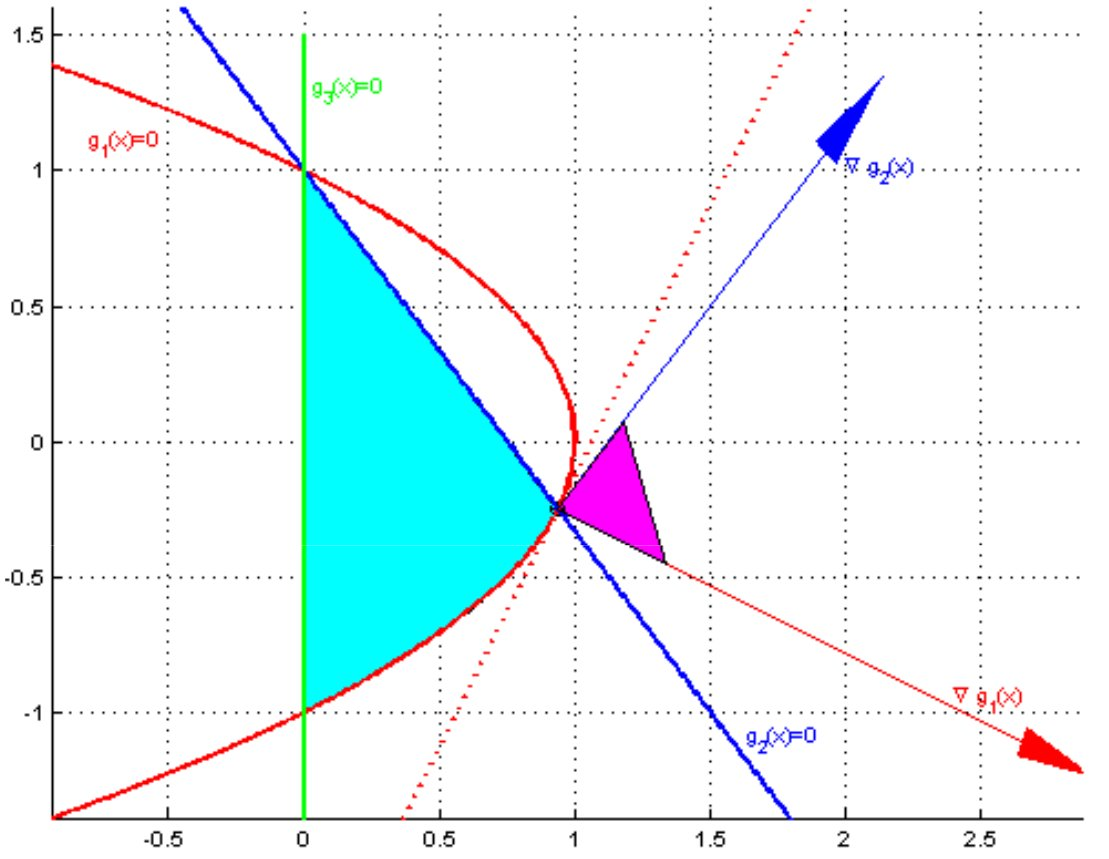
\includegraphics[scale=0.5]{constrained_opt}\caption{Inequality constrained feasible region\label{fig:Inequality-constrained-feasible}}

\par\end{centering}

\end{figure}

\end{example*}
Note a trick: we can make any feasible $\bar{x}$ point to some minimization
problem a Fritz-John point of a related system by adding the constraints
$\left\lVert x-\bar{x}\right\rVert ^{2}\geq0$. 
\begin{thm*}
KKT conditions. Suppose all the conditions of Fritz-John are met and
$\nabla g_{I}\left(\bar{x}\right)$ are linearly independent. Then
\begin{align*}
\nabla f\left(\bar{x}\right)+\sum_{i=1}^{m}u_{i}\nabla g_{i}\left(\bar{x}\right) & =0\\
u_{i}g_{i}\left(\bar{x}\right) & =0\\
u_{i} & \geq0
\end{align*}
\end{thm*}
\begin{proof}
By Fritz-John there exist 
\begin{align*}
u_{0}\nabla f\left(\bar{x}\right)+\sum_{i=I}u_{i}\nabla g_{i}\left(\bar{x}\right) & =0\\
u_{0},u_{I} & \geq0\\
\left(u_{0},u_{I}\right) & \neq\left(0,0\right)
\end{align*}
and $u_{0}>0$ since otherwise $\left\{ \nabla g_{i}\left(\bar{x}\right)\right\} $
would be linearly dependent. Hence dividing by $u_{0}$ we get the
conclusion.
\end{proof}
Connection of KKT to first-order LP approximations to NLPs:
\begin{thm*}
Let $X$ be nonempty open. Consider 
\[
\min\left\{ f\left(x\right)\big|x\in X,g_{i}\left(x\right)\leq0,i\in M=\left\{ 1,\dots,m\right\} \right\} 
\]
with $f,g_{i}$ differentiable. Let $\bar{x}$ be feasible and $g_{I}\left(\bar{x}\right)=0$.
Let $F_{0},G_{0}^{'}=\left\{ d\neq0\big|\nabla g_{I}\left(\bar{x}\right)^{t}d\leq0\right\} ,G^{'}=G^{'}\cup\left\{ 0\right\} $.
Then $\bar{x}$ is $KKT$ iff $F_{0}\cap G^{'}=\emptyset\iff F_{0}\cap G_{0}^{'}=\emptyset$.
Further $\bar{x}$ is KKT iff 
\[
\bar{x}=\min_{x}\left\{ f\left(\bar{x}\right)+\nabla f\left(\bar{x}\right)^{t}\left(x-\bar{x}\right)\big|g_{I}\left(\bar{x}\right)+\nabla g_{I}\left(\bar{x}\right)^{t}\left(x-\bar{x}\right)\leq0\right\} 
\]

\end{thm*}

\begin{thm*}
Sufficient conditions for KKT point to be locally optimal. If $\bar{x}$
is a KKT solution and there exists a neighborhood $\mathcal{N}_{\epsilon}\left(\bar{x}\right)$
such that $f$ is convex over $\mathcal{N}_{\epsilon}\left(\bar{x}\right)\cap S$,
the $g_{I}$ are differentiable and convex over $\mathcal{N}_{\epsilon}\left(\bar{x}\right)\cap S$,
then $\bar{x}$ is a local minimum.
\end{thm*}

\begin{thm*}
Sufficient conditions for KKT point to be globally optimal. If 
\[
\min\left\{ f\left(x\right)\big|x\in X,g_{i}\left(x\right)\leq0,i\in M=\left\{ 1,\dots,m\right\} \right\} 
\]


is convex (i.e. $f,g_{i}$ are convex everywhere) and $\bar{x}$ is
a KKT point. Then $\bar{x}$ is globally optimal.
\end{thm*}
Note that not every every globally optimal point of a convex program
is a KKT point. Also if the constraints are equalities then the multipliers
are free (not necessarily positive) and if the constraints are greater
than then the multipliers are negative.


\subsection{Second order conditions for local optimality }

Consider the problem
\begin{align*}
\min & \,f\left(x\right)\\
\text{s.t.} & g_{I}\left(x\right)\leq0\\
 & h_{J}\left(x\right)=0
\end{align*}

\begin{defn*}
The \emph{Lagrangian }is 
\[
L\left(x,u,v\right)=f\left(x\right)+\sum_{i\in I}u_{i}g_{i}\left(x\right)+\sum_{j\in J}v_{j}h_{j}\left(x\right)
\]
\end{defn*}
\begin{thm*}
Sufficient conditions. Suppose $\bar{x}$ is a KKT point with Lagrange
multipliers $\bar{u},\bar{v}$. Then
\begin{enumerate}
\item If $\nabla L^{2}\left(x\right)=\nabla L^{2}\left(x,\bar{u},\bar{v}\right)$
is psd for all $x\in S$, then $\bar{x}$ is a global minimum.
\item If $\nabla L^{2}\left(x\right)=\nabla L^{2}\left(x,\bar{u},\bar{v}\right)$
is psd for all $x\in\mathcal{N}_{\epsilon}\left(\bar{x}\right)\cap S$,
then $\bar{x}$ is a local minimum.
\item If $\nabla L^{2}\left(x\right)=\nabla L^{2}\left(x,\bar{u},\bar{v}\right)$
is pd then $\bar{x}$ is a strict local minimum.
\end{enumerate}
\end{thm*}

\begin{thm*}
Necessary conditions. Suppose $\bar{x}$ is a local minimum Lagrange
multipliers $\bar{u},\bar{v}$ and $\nabla g_{I}\left(\bar{x}\right)$
(where $I$ is the set of binding constraints) are linearly independent
and $\nabla h_{J}\left(\bar{x}\right)$ are linearly independent.
Then $\bar{x}$ is a KKT point having Lagrange multipliers $\bar{u}\geq0$
and $\nabla^{2}L\left(\bar{x}\right)$ is psd over
\[
C=\left\{ d\neq0\bigg|\begin{array}{cc}
\nabla g_{I^{+}}\left(\bar{x}\right)^{t}d=0 & I^{+}=\left\{ i\in I\big|\bar{u}_{i}\geq0\right\} \\
\nabla g_{I^{0}}\left(\bar{x}\right)^{t}d\leq0 & I^{0}=\left\{ i\in I\big|\bar{u}_{i}=0\right\} \\
\nabla h_{J}\left(\bar{x}\right)^{t}d=0
\end{array}\right\} 
\]

\end{thm*}

\begin{thm*}
Let $\bar{x}$ be a KKT point. If $\nabla^{2}L\left(\bar{x}\right)$
is pd over $C$ then $\bar{x}$ is a strict local minimum.
\end{thm*}
In summary

\noindent \begin{center}
\begin{table}


\noindent \begin{centering}
\begin{tabular}{|c|c|c|}
\hline 
 & Unconstrained & Constrained\tabularnewline
\hline 
\hline 
Problem & $\min\,f\left(x\right)$ & 
\begin{align*}
\min & \,f\left(x\right)\\
\text{s.t.} & g_{i}\left(x\right)\leq0\\
 & h_{i}\left(x\right)=0
\end{align*}
\tabularnewline
\hline 
First Order & $\nabla f\left(x\right)=0$ & 
\begin{align*}
\nabla_{x,v}L\left(x,\bar{u},v\right) & =0\\
\lambda_{i}g_{i}\left(x\right) & =0\\
\lambda_{i} & \geq0
\end{align*}
\tabularnewline
\hline 
Second order necessary & $\nabla^{2}f\left(x\right)$ psd & $\nabla^{2}L\left(x\right)$ psd for all $d\in C$\tabularnewline
\hline 
Second order sufficient & $\nabla^{2}f\left(x\right)$ pd & $\nabla^{2}L\left(x\right)$ pd for all $d\in C$\tabularnewline
\hline 
\end{tabular}\caption{Optimality conditions summary}

\par\end{centering}

\end{table}

\par\end{center}


\section{Lagrangian Duality}
\begin{defn*}
Consider the following related pair of optimization problems

\begin{align*}
z^{P} & =\min\left\{ f\left(x\right)\big|x\in X\right\} \\
z^{R} & =\min\left\{ g\left(x\right)\big|x\in Y\right\} 
\end{align*}
$R$ is a \emph{relaxation} of $P$ if $f\left(x\right)\geq g\left(x\right)$
for all $x\in X$ and $X\subset Y$.\end{defn*}
\begin{thm*}
Let $R$ be a relaxation of $P$
\begin{enumerate}
\item If $R$ is infeasible then so is $P$.
\item If $P$ and $R$ have optimal solutions then $z^{P}\geq z^{R}$
\item If $x^{R}$ is an optimal solution to $R$ such that $x^{R}\in X$
and $g\left(x^{R}\right)=f\left(x^{R}\right)$, then $x^{R}$ is an
optimal solution for $P$.
\end{enumerate}
\end{thm*}
\begin{defn*}
Consider the primal optimization problem
\begin{align*}
\min & \,f\left(x\right)\\
\text{s.t.} & g_{i}\left(x\right)\leq0\text{ for all }i=1,\dots,m\\
 & h_{j}\left(x\right)=0\text{ for all }j=1,\dots,n\\
 & x\in X
\end{align*}
The Lagrangian dual is
\begin{align*}
\max & \,\theta\left(u,v\right)\\
\text{s.t.} & u\in\mathbb{R}_{+}^{m},v\in\mathbb{R}^{n}
\end{align*}
where 
\[
\theta\left(u,v\right)=\min_{x}\,L\left(x,u,v\right)
\]
where
\[
L\left(x,u,v\right)=f\left(x\right)+\sum_{i=1}^{m}u_{i}g_{i}\left(x\right)+\sum_{j=1}^{n}v_{j}h_{j}\left(x\right)
\]
\end{defn*}
\begin{example*}
Consider the problem

\begin{align*}
\min & \,x_{1}^{2}+x_{2}^{2}\\
\text{s.t.} & -x_{1}-x_{2}+4\leq0\\
 & x_{1},x_{2}\geq0
\end{align*}
''Dualize'' the first constraint: 
\[
L\left(u,x_{1},x_{2}\right)=x_{1}^{2}+x_{2}^{2}+u\left(-x_{1}-x_{2}+4\right)
\]
Then the dual function is 
\begin{align*}
\theta\left(u\right) & =\min_{x_{1},x_{2}}\,L\left(u,x_{1},x_{2}\right)\\
 & =\min_{x_{1},x_{2}}\,\left(x_{1}^{2}-ux_{1}+x_{2}^{2}-ux_{2}+4u\right)\\
 & =4u+\min_{x_{1}\ge0}\,\left(x_{1}^{2}-ux_{1}\right)+\min_{x_{2}\ge0}\,\left(x_{2}^{2}-ux_{2}\right)\\
 & =4u+\left\{ \begin{alignedat}{1}-\frac{u^{2}}{4} & \text{ if }u\geq0\\
0 & \text{ if }u<0
\end{alignedat}
\right\} +\left\{ \begin{alignedat}{1}-\frac{u^{2}}{4} & \text{ if }u\geq0\\
0 & \text{ if }u<0
\end{alignedat}
\right\} \\
 & =\left\{ \begin{alignedat}{1}4u-\frac{u^{2}}{2} & \text{ if }u\geq0\\
4u & \text{ if }u<0
\end{alignedat}
\right\} 
\end{align*}

\end{example*}

\subsection{A general procedure for deriving duals}

Procedure:
\begin{enumerate}
\item Build the Lagrangian function (choose the appropriate constraints
to ``dualize'').
\item For fixed Langrange multipliers do the minimization (or maximization).
\item Simplify the description of the Lagrangian.
\item Express the dual.
\end{enumerate}

\subsection{Deriving duals}
\begin{example*}
The Langrangian dual of the QP 
\[
\min\left\{ d^{t}x+\frac{1}{2}x^{t}Hx\big|Ax\preceq b\right\} 
\]
where $H$ is pd and symmetric is 
\[
\max\left\{ \frac{1}{2}u^{t}Du+u^{t}C-\frac{1}{2}d^{t}H^{-1}d\big|u\succeq0\right\} 
\]
where $D=-AH^{-1}A^{t},C=-b-AH^{-1}d$. Why? 
\begin{enumerate}
\item Build the Lagrangian
\begin{align*}
L\left(u\right) & =\min_{x\in\mathbb{R}^{n}}\left\{ d^{t}x+\frac{1}{2}x^{t}Hx+u^{t}\left(Ax-b\right)\right\} \\
 & =\min_{x\in\mathbb{R}^{n}}\left\{ \frac{1}{2}x^{t}Hx+\left(d^{t}+u^{t}A\right)x-u^{t}b\right\} \\
 & =-u^{t}b+\min_{x\in\mathbb{R}^{n}}\left\{ \frac{1}{2}x^{t}Hx+\left(d^{t}+u^{t}A\right)x\right\} 
\end{align*}

\item For a fixed $u$ the inner minimization is convex and unconstrained,
so we can use first order conditions: solve for $x$
\[
Hx+\left(d^{t}+u^{t}A\right)=0
\]
i.e. $x^{*}=-H^{-1}\left(d+A^{t}u\right)$
\item Simplifying $L\left(u\right)$ we get
\[
L\left(u\right)=-\frac{1}{2}d^{t}H^{-1}d+u^{t}\left(-b-AH^{-1}d\right)-\frac{1}{2}u^{t}AH^{-1}A^{t}u
\]

\item Express the dual
\[
\max\left\{ \frac{1}{2}u^{t}Du+u^{t}C-\frac{1}{2}d^{t}H^{-1}d\big|u\succeq0\right\} 
\]
Note that $u\succeq0$ because $Ax-b\preceq0$ and hence $u$s should
be positive in order for $u\left(Ax-b\right)$ to be a relaxation.
\end{enumerate}
\end{example*}
\begin{defn*}
Given a closed convex cone $K\subset\mathbb{R}^{n}$, the \emph{dual
cone} $K^{*}$ of $K$
\[
K^{*}=\left\{ y\in\mathbb{R}^{n}\big|y^{t}x\geq0,\forall x\in K\right\} 
\]
I.e. all vectors that make an acute angle with every vector in $K$.\end{defn*}
\begin{example*}
Some cones are ``self-dual''
\begin{enumerate}
\item $\left(\mathbb{R}_{+}^{n}\right)^{*}=\mathbb{R}_{+}^{n}$
\item $\left(\mathcal{C}_{n}\right)^{*}=\mathcal{C}_{n}$ where $\mathcal{C}_{n}$
is the $n$ dimensional second order cone.
\item $\left(S_{+}^{n\times n}\right)^{*}=S_{+}^{n\times n}$ where $S_{+}^{n\times n}$
is the cone of $n\times n$ psd matrices.
\end{enumerate}
\end{example*}
\begin{thm*}
If $K$ is a nonempty closed convex cone then so is $K^{*}$.\end{thm*}
\begin{example*}
The Lagrangian dual of the conic LP
\[
\min\left\{ c^{t}x\big|Ax=b,x\in K\right\} 
\]
is
\[
\max\left\{ b^{t}v\big|A^{t}v+s=c,s\in K^{*}\right\} 
\]


Why?
\begin{enumerate}
\item Build the Lagrangian dual
\begin{align*}
L\left(v\right) & =\min_{x\in K}\ c^{t}x+v^{t}\left(b-Ax\right)\\
 & =v^{t}b+\min_{x\in K}\ \left(c^{t}-v^{t}A\right)x
\end{align*}

\item For a fixed $u$ this is optimizing a linear function over a cone
$K$, therefore the problem will be bounded iff
\[
c-A^{t}v\in K^{*}
\]
(otherwise we could just ``runaway''). Similarly as in the straightforward
LP case we have that if there is an optimal solution it's at 0. 
\item Simplify the Lagrangian
\[
L\left(v\right)=\begin{cases}
b^{t}v & \text{ if }c-A^{t}v\in K^{*}\\
-\infty & \text{ if }c-A^{t}v\not\in K^{*}
\end{cases}
\]

\end{enumerate}
\end{example*}
\begin{thm*}
The dual of the dual of the conic LP
\[
\min\left\{ c^{t}x\big|Ax=b,x\in K\right\} 
\]
is
\[
\min\left\{ c^{t}x\big|Ax=b,x\in\left(K^{*}\right)^{*}\right\} 
\]

\end{thm*}

\begin{thm*}
If $K$ is a nonempty closed convex cone then $\left(K^{*}\right)^{*}=K$.
\end{thm*}

\subsection{The strength of duals}
\begin{thm*}
Weak duality. Let $x$ be a feasible solution to a primal problem
and $\left(u,v\right)$ be a feasible solution to the dual. Then $f\left(x\right)\geq L\left(u,v\right)$.\end{thm*}
\begin{cor*}
The optimal solution to the primal is greater or equal to the optimal
solution to the dual.
\end{cor*}

\begin{cor*}
If $\bar{x}$ and $\left(\bar{u},\bar{v}\right)$ are such that $f\left(\bar{x}\right)=L\left(\bar{u},\bar{v}\right)$
then $\bar{x}$ solves the primal and $\left(\bar{u},\bar{v}\right)$
solves the dual.
\end{cor*}

\begin{cor*}
If the primal is unbounded then $L\left(u,v\right)=-\infty$ for all
$u,v$.
\end{cor*}

\begin{cor*}
If the dual is unbounded then the primal is infeasible.\end{cor*}
\begin{defn*}
When the optimal solution to the primal and the optimal solution to
the dual differ there's a duality gap.\end{defn*}
\begin{lem*}
Let $X$ be a nonempty convex subset of $\mathbb{R}^{n}$, $\alpha:\mathbb{R}^{n}\rightarrow\mathbb{R}$,
$g:\mathbb{R}^{n}\rightarrow\mathbb{R}^{m}$ convex functions and
$h=Ax-b$. 

\begin{align*}
\left\{ \alpha<0,g\left(x\right)\leq0,h\left(x\right)=0\right\}  & =\emptyset\\
 & \Rightarrow\\
\left\{ u_{0}\alpha\left(x\right)+u^{t}g\left(x\right)+v^{t}h\left(x\right)\geq0,\forall x\in X,\left(u_{0},u\right)\geq0,\left(u_{0},u,v\right)\neq0\right\}  & \neq\emptyset
\end{align*}
The converse holds if $u_{0}>0$.\end{lem*}
\begin{thm*}
Strong Duality. There is no duality gap if there exists $\hat{x}\in X$
such that $g\left(\hat{x}\right)<0,h\left(\hat{x}\right)=0,0\in\text{int}\left(h\left(X\right)\right)$\end{thm*}
\begin{defn*}
A \emph{saddle point of the Lagrangian is $\left(\bar{x},\bar{u},\bar{v}\right)$
such that 
\[
L\left(\bar{x},u,v\right)\leq L\left(\bar{x},\bar{u},\bar{v}\right)\leq L\left(x,\bar{u},\bar{v}\right)
\]
}\end{defn*}
\begin{thm*}
A solution $\left(\bar{u},\bar{v},\bar{x}\right)$ with $\bar{u}\geq0$
is a saddle point for the Lagrangian iff
\begin{enumerate}
\item $L\left(\bar{u},\bar{v},\bar{x}\right)=\min\left\{ L\left(\bar{u},\bar{v},x\right)\right\} $
\item $g\left(\bar{x}\right)\le0$ and $h\left(\bar{x}\right)=0$
\item $\bar{u}^{t}g\left(\bar{x}\right)=0$
\item $\bar{x}$ and $\left(\bar{u},\bar{v}\right)$ are optimal for the
primal problem and the dual problem respectively and there's no duality
gap.
\end{enumerate}
\end{thm*}
Fact: the dual function is always concave and it's differentiable
when something something something is unique.
\end{document}
